\documentclass[12pt]{article}
        \usepackage{graphicx,type1cm,eso-pic,color}
        \usepackage{hyperref}
        \usepackage[left=3.0cm,right=3.0cm,top=2cm,bottom=2cm,headheight=13.6pt]{geometry}
        \usepackage{subfigure}

\makeatother


\title{Manual for CLAS12 \\ Ring Imaging Cherenkov Counter}

\author{RICH On-Call Cell Phone: 757-810-1489 \\ 
Authors: \\
M. Contalbrigo (mcontalb@jlab.org) \\
V. Kubarovsky (vpk@jlab.org)\\
M. Mirazita (mirazita@jlab.org)\\
}

\date{\today} %01/07/2014


\begin{document}
\maketitle{}

\tableofcontents

%%%%%%%%%%%%%%%%%%%%%%%%%%%%%%%%%%%%%%%%%%%%%%%%%%%%%%%%%%%%%%%
\newpage
   \section{General description of the RICH}

The first module of the CLAS12 Ring Imaging CHerenkov (RICH) detector is installed on the forward carriage in Sector 4, downstream of the third region of drift chambers and just before the Time-Of-Flight (TOF) system.
A second RICH module is foreseen for the starting of operation with transversely polarized target.
It's goal is to provide identification of kaons with respect to pions and protons at a 4~$\sigma$ level in the momentum range between 3 and 8 GeV/c for polar angles up to 35$^o$.
The RICH design incorporates aerogel radiators, visible light photon detectors, and a focusing mirror system which is used to reduce the detection area instrumented by photon detectors to about 1 m$^2$. 
Multi-anode photomultiplier tubes (MAPMTs) Hamamatsu H8500 and H12700 provide the required spatial resolution and match the aerogel Cherenkov light spectrum (visible and near-ultraviolet region). 

The RICH is composed by a large trapezoidal box made in aluminum and carbon fiber, with smaller base of about 0.3 m, a larger base of about 4.2 m, a height of about 3.7 m and a depth of about 1.2 m. 
The total weight is approximately 900 Kg. 
Two drawings of the RICH box frontal and backward views are shown in figure~\ref{fig:RICH_outer}. 


\vspace*{\stretch{1}}      
\begin{figure}[h!]
\center
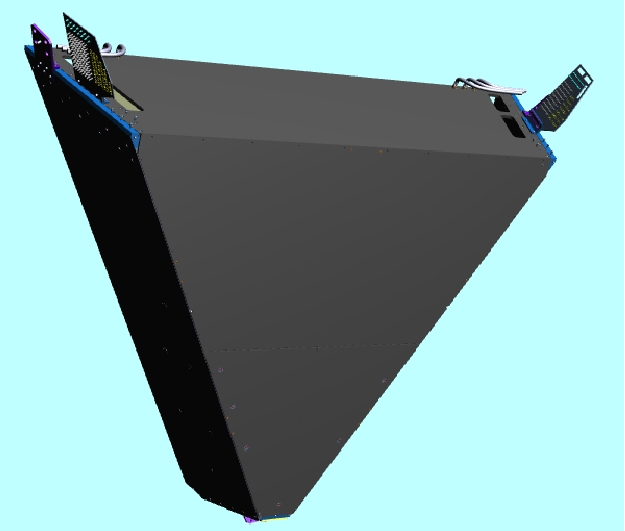
\includegraphics[width=0.53\textwidth]{Rich_frontal.jpg}
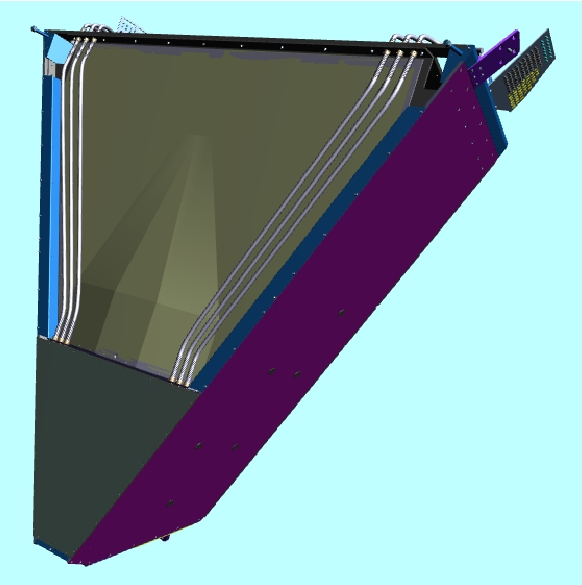
\includegraphics[width=0.46\textwidth]{Rich_back.jpg}
\caption{ \label{fig:RICH_outer} Back and frontal drawings of the RICH module.}
\end{figure}

Inside the RICH box, a number of active elements are installed, namely:
\begin{itemize}
\item{the aerogel radiator;}
\item{the planar and spherical mirrors;}
\item{the MAPMTs and the readout Front-End Electronics (FEE).}
\end{itemize}

A cross section of the RICH showing the inner elements in shown in figure~\ref{fig:RICH_inner}.

\vspace*{\stretch{1}}      
\begin{figure}[h!]
\center
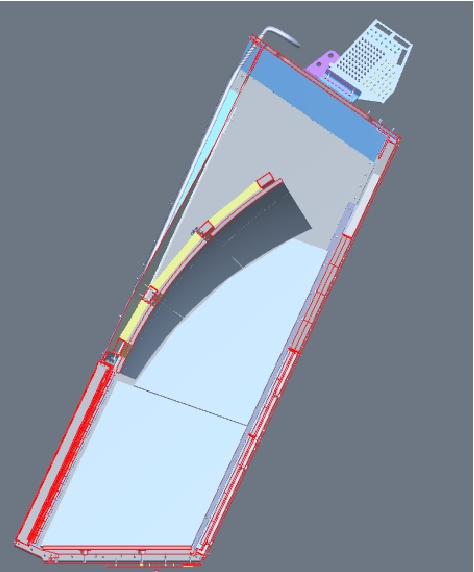
\includegraphics[width=0.9\textwidth]{Rich_lateral.jpg}
\caption{ \label{fig:RICH_inner} Cross section of the RICH.}
\end{figure}

The aerogel is an igrophilic material that absorbs water from the environment humidity, resulting in a reduction of its optical performance.
For this reason, a strict protocol to handle it has been established during the test and assembly.
In addition, the RICH box volume is fluxed with dry nitrogen, in order to prevent water absorption during the operation of the detector.

The detection of the Cherenkov photon is achieved by means of 391 Hamamatsu H8500 and H12700 MAPMTs, mounted on a triangular box, about 1.7 m wide, 1.3 m high and about 10 cm thick, that is installed on the lower back of the RICH module.
The FEE is organized in tiles serving groups of two or three MAPMTs.
Each tile is composed by an adapter board, an ASIC board housing the MAROC3 chip for the MAPMT readout and an FPGA in charge to configure the chip and to ensure the connection with the DAQ systems via optical link.
There is one MAROC3 chip per MAPMT and one FPGA per tile.
The total number of tiles is 138.


%%%%%%%%%%%%%%%%%%%%%%%%%%%%%%%%%%%%%%%%%%%%%%%%%%%%%%%%%%%%%%%
%\newpage
{\color{blue}
\section{The RICH Gas Systems}
}

The RICH is serviced by two different gas systems, one for the supply of the nitrogen to be fluxed inside the RICH box and one for the cooling of the FEE.
Both systems are managed through controls and monitors integrated in the CLAS12 software.
The two systems have been dimensioned in such a way that they will be able to serve two RICH modules.


%=============================================================
\subsection{The Nitrogen System}

In order to preserve the aerogel optical performance, the RICH box environment must be kept dry by fluxing nitrogen.
The nitrogen system supplies the amount of gas necessary to fill the box (about 6 cubic meters) and to compensate for the gas leakage.
A complete refill of the volume per day is expected under normal operating conditions.
A slight overpressure of 0.5 mbar prevents from the contamination from the outside air.
The system is shown in Fig. \ref{fig:N2_drawing}.
It is based on a 1500 Gallons dewar of liquid nitrogen connected to the RICH box through a on/off valve with a pressure regulator, a 0.01 micron filter to remove all the impurities and flow-meters.
In figure \ref{fig:N2_components}, we report the list of the components of the system.

\vspace*{\stretch{1}}      
\begin{figure}[h!]
\center
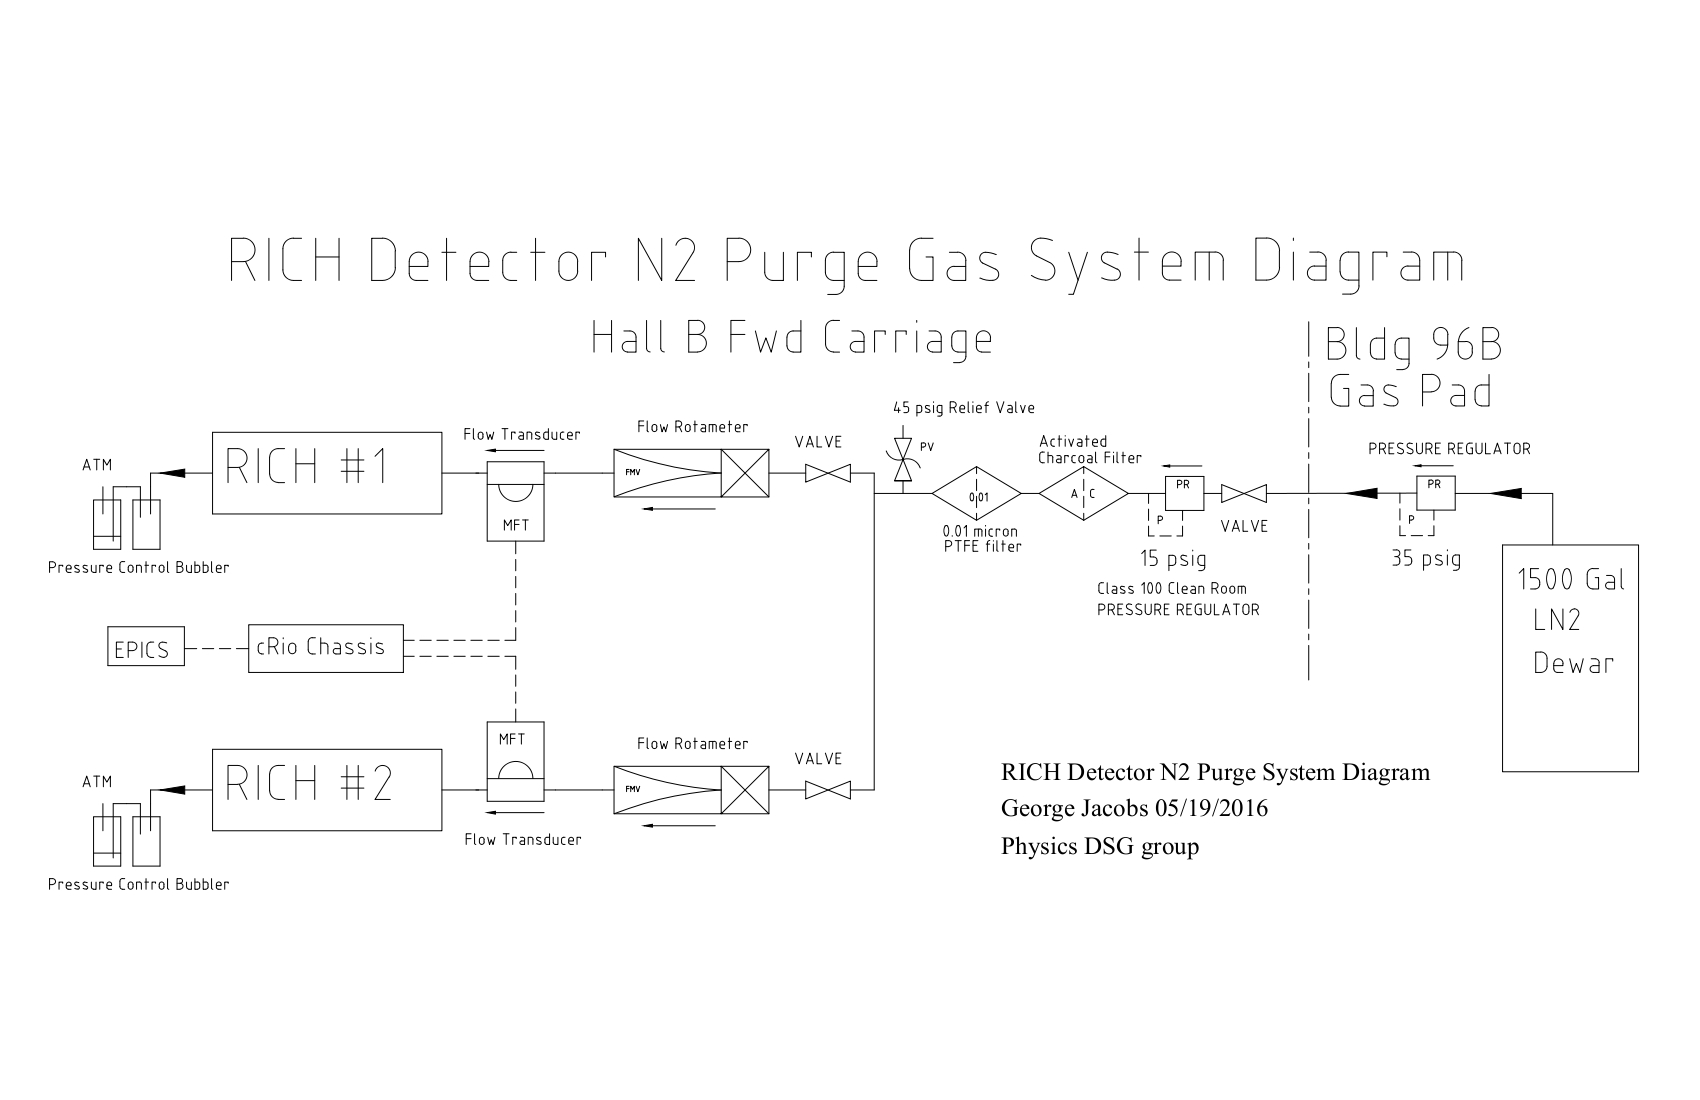
\includegraphics[width=0.95\textwidth]{N2_drawing.jpg}
\caption{ \label{fig:N2_drawing} Schematic of the nitrogen supply system.}
\end{figure}

\vspace*{\stretch{1}}      
\begin{figure}[h!]
\center
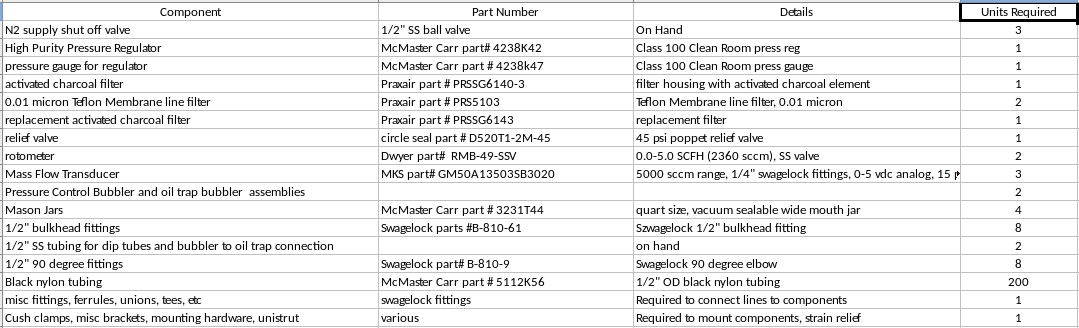
\includegraphics[width=0.95\textwidth]{N2_components.jpg}
\caption{ \label{fig:N2_components} Complete list of the components of the nitrogen supply system.}
\end{figure}



The slow control checks online the correct functionality of the system, i.e.:
\begin{itemize}
\item{Minimum pressure in the liquid nitrogen dewar;}
\item{Minimum flow inside the RICH box;}
\item{Purity of the gas fluxed inside the RICH box.}
\end{itemize}
In the case of failure of the purity control, the valve is automatically turned off and the flow stopped, to prevent possible damage to the aerogel.



%=============================================================
\subsection{The Cooling System}

One tile with two or three MAPMs produces about 3.35 or 3.8 W of heat load, respectively.
The total load in the whole FEE box is 514 W.
This heat load must be dissipated far from the CLAS12 detectors in order to keep the FEE box temperature below 40 $^o$C, the safety limit imposed by the TOF detector which is few cm downstream of the RICH.
%Laboratory have shown that a proper cooling of the system can be obtained by fluxing about 200 liter /min of compressed air.

The FEE RICH cooling system is based on two high capacity air compressors that supply clean dry air at room temperature.
The minimum capacity of each compressor must be 600 l/min, so that, in case of failure of one of the two, the other has sufficient capacity to supply the necessary cooling power to two RICH modules.
The compressors charge a 1000 liter capacity air tank.
Air pressure is reduced to supply manual valve flow meters.
In the case of a power outage, the air tank should contain sufficient air to remove the latent heat of the FEE package.
The characteristics of the compressors are shown in table \ref{tab:Compressor}.

\begin{table}[htbp]\centering
    \begin{tabular}{||c|l||}
\hline
\hline
Dimensions & 1.4 x 0.7 x 1.8 m$^3$ \\
\hline
Weight & 515 kg \\
\hline
Max Flow rate  & 1200 l/min \\
\hline
Dew point & 3 $^o$C \\
\hline
Electric power & 10.4 kW \\
\hline
Noise press & 60 dB (A) \\
\hline
\hline
    \end{tabular}
    \caption{The characteristics of the ATLAS Copco SF11-8 MC FF compressors. \label{tab:Compressor}}
\end{table}



Powering up the electronics package inside the RICH without cooling may result in severe damage of the RICH and of other detectors or even fire.
To eliminate this hazard, the RICH HV and LV power supply operations are interlocked to the proper functioning of the cooling system.

A schematic of the RICH cooling system with the interlock circuits is shown in figure \ref{fig:Cooling_interlocks} and the list of its components is reported in figure \ref{fig:Cooling_components}.
It includes a number of temperature sensors installed inside the electronics box, air flow transducers and high purity pressure regulators connected to the inlets and a local pressure regulators on the air tank.
The interlock performs two functions in case of a cooling system failure.
\begin{itemize}
\item{turn off power to the electronic package;}
\item{prevent energizing the electronics package.}
\end{itemize}
There are three cooling cicuit interlocks.
A first interlock requires the minimum of one compressor correctly functioning.
The second interlock requires a minimum air pressure in the tank.
The third interlock require a minimum air flow inside the RICH box.
All three interlocks must be true in order for the electronics package to have power.

\vspace*{\stretch{1}}      
\begin{figure}[h!]
\center
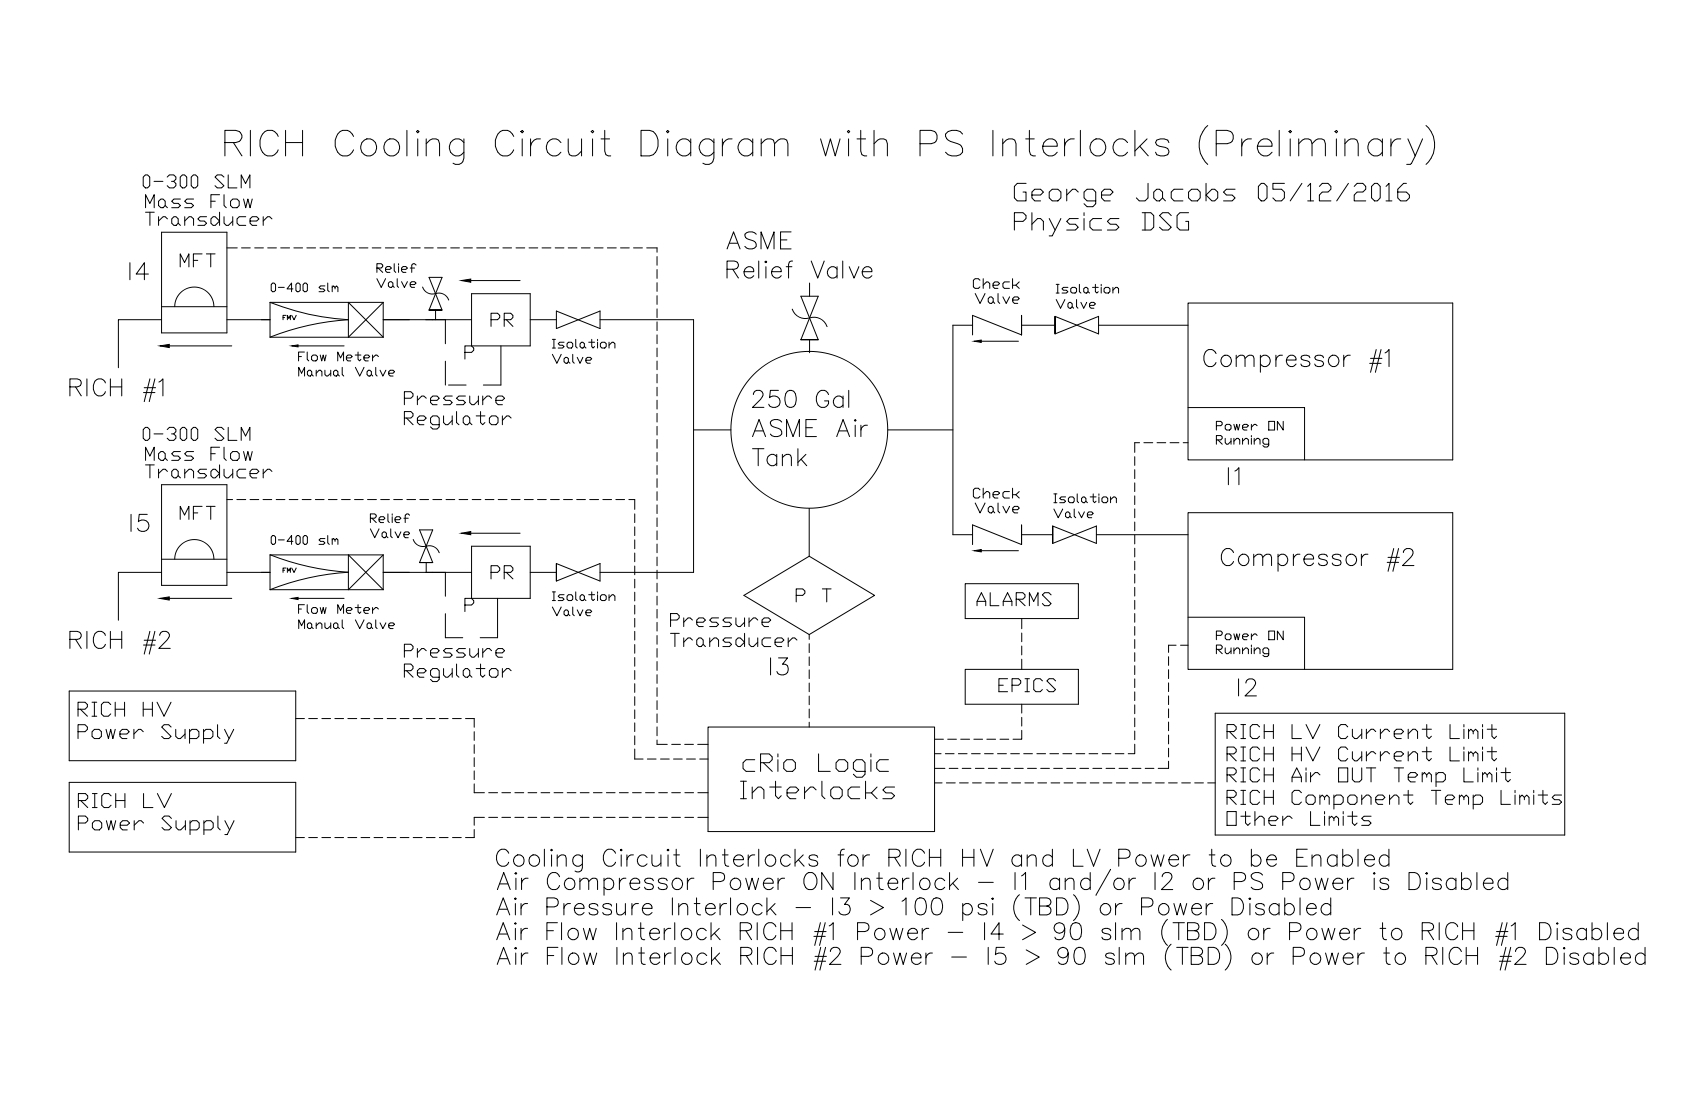
\includegraphics[width=0.9\textwidth]{Cooling_interlocks.jpg}
\caption{ \label{fig:Cooling_interlocks} Schematic of the cooling system and interlocks.}
\end{figure}

\vspace*{\stretch{1}}      
\begin{figure}[h!]
\center
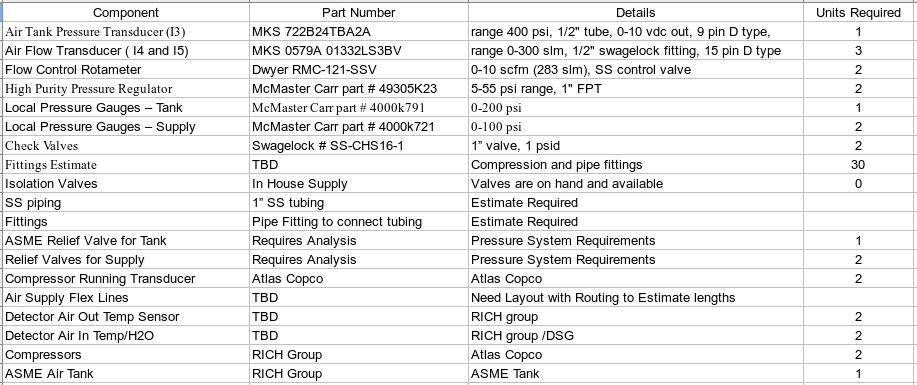
\includegraphics[width=0.9\textwidth]{Cooling_components.jpg}
\caption{ \label{fig:Cooling_components} Complete list of the components of the cooling system and interlocks.}
\end{figure}


%%%%%%%%%%%%%%%%%%%%%%%%%%%%%%%%%%%%%%%%%%%%%%%%%%%%%%%%%%%%%%

{\color{blue}
 \twocolumn
\part{Shift Takers Instructions}
}
\vspace*{\stretch{1}}      
All RICH controls will be  accessible through EPICS, from the main CLAS\_EPICS window (figure~\ref{EPICSmain}).  If not already running, it can be opened by executing
the command 
\begin{center}
\texttt{clas\_epics}
\end{center}
 in a terminal on any of the \texttt{clonpc\#\#} workstations in the Hall-B counting house.

{\em   All shift workers should be using user \texttt{clasrun} for all instructions in this document.}

The primary RICH screen is shown in figure~\ref{fig:ecal_all} and opened via the {\bf RICH} button in the right side of the main CLAS EPICS screen (figure~\ref{EPICSmain}).

From the main CLAS\_EPICS window you can also access individual screens with more controls and details, {\bf Temperature monitoring} in {\it Miscellaneous} then {\it RICH Temperature}, the {\bf RICH chiller} in {\it Devices} then {\it Chiller (RICH)}, the {\bf Scalers} in {\it RICH Scaler GUI}, the {\bf RICH high voltage} in {\it Voltages} then {\it RICH HV}.


\vspace*{\stretch{1}}      
\begin{figure}[h!]
\center
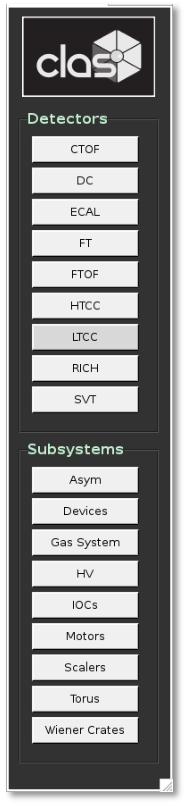
\includegraphics[width=0.28\textwidth]{pics/CLAS_EPICS.pdf}
%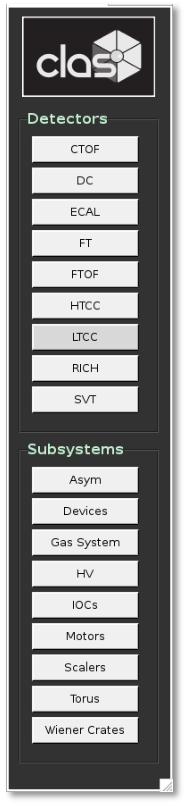
\includegraphics[width=0.38\textwidth]{pics/CLAS_EPICS.pdf}
%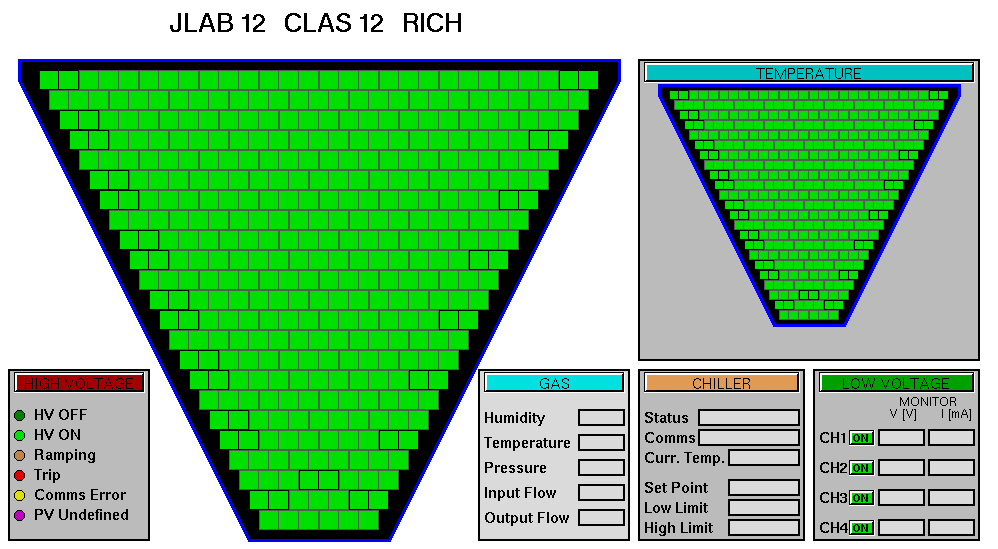
\includegraphics{pics/ElectronicPanel.png}
\caption{ \label{EPICSmain} View of the Hall-B EPICS main window.}
\end{figure}

 \onecolumn

{\color{blue}

 \section{Primary RICH EPICS Screen}
}
 This one screen combines all basic RICH EPICS controls and monitoring into one window.  It is accessible from the {\bf RICH} button in figure~\ref{EPICSmain}.  This includes embedded versions of the dedicated screens in the following sections:  temperature sensors, chiller, and low and high voltage.  
 
 This screen provides the only RICH {\em controls} shift workers should need, which is to turn HV on and off via the red and green {\bf ALL ON} and {\bf ALL OFF} buttons.  However, this should be supplemented by the strip charts for temperature and HV current, as well as cctv webcams, for additional {\em monitoring} in the following sections.

The grey square buttons in the top right of each section of this main RICH screen provide
access to more detailed or expert screens for the corresponding subsystem.


\begin{figure}[htbp]\centering
    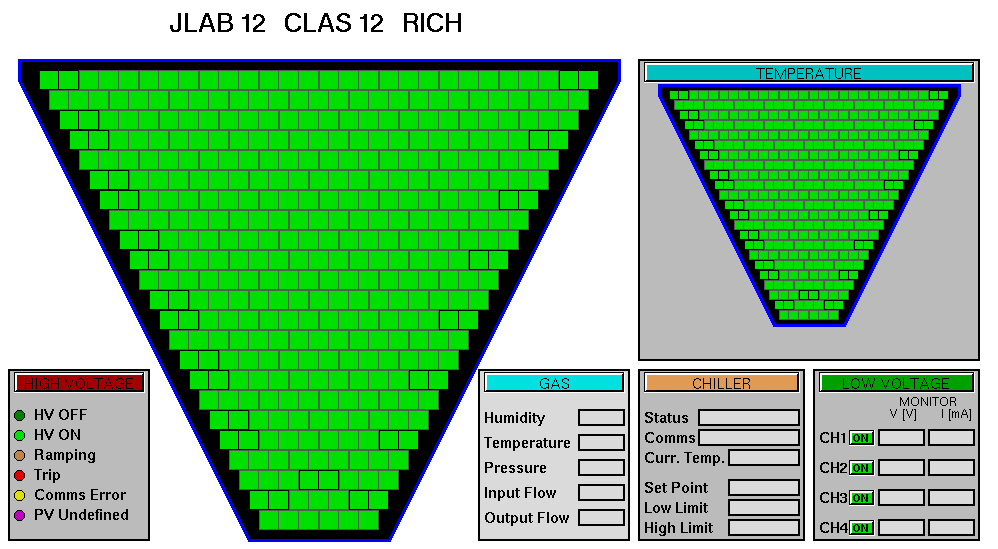
\includegraphics[width=15.5cm]{pics/ElectronicPanel.png}
    \caption{The primary EPICS screen needed for shift workers to monitor RICH.\label{fig:ecal_all}}
\end{figure}


\newpage
{\color{blue}
\section{Temperature}
}
The RICH temperature should remain stable.  Cooling controls and monitoring are described in this section.

\subsection{Temperature Sensors}
Eighteen temperature sensors are placed in the RICH enclosure and should be monitored through RICH's main EPICS screen and the strip charts shown in in figure~\ref{temp2}. Variations of two degrees F or more during a shift should be reported to RICH expert on call and noted in the log book.  The strip charts are accessible from the two buttons in the temperature section of Figure ~\ref{fig:ecal_all} (and also the main CLAS\_EPICS screen in Figure \ref{EPICSmain}).
%\begin{figure}[htbp]
%\center
%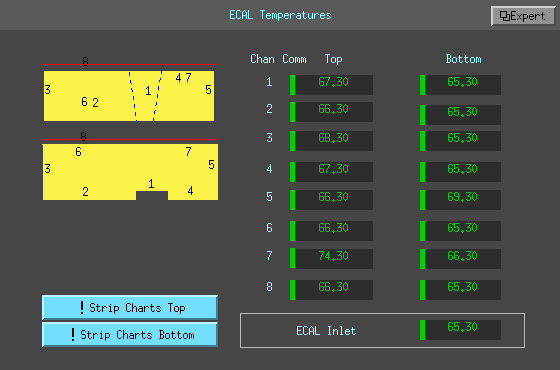
\includegraphics[width=0.5\textwidth]{pics/EcalTemp_2014_12_20.png}
%\caption{ \label{temp} View of the EPICS temperature monitoring window.}
%\end{figure}
\begin{figure}[htbp]
\center
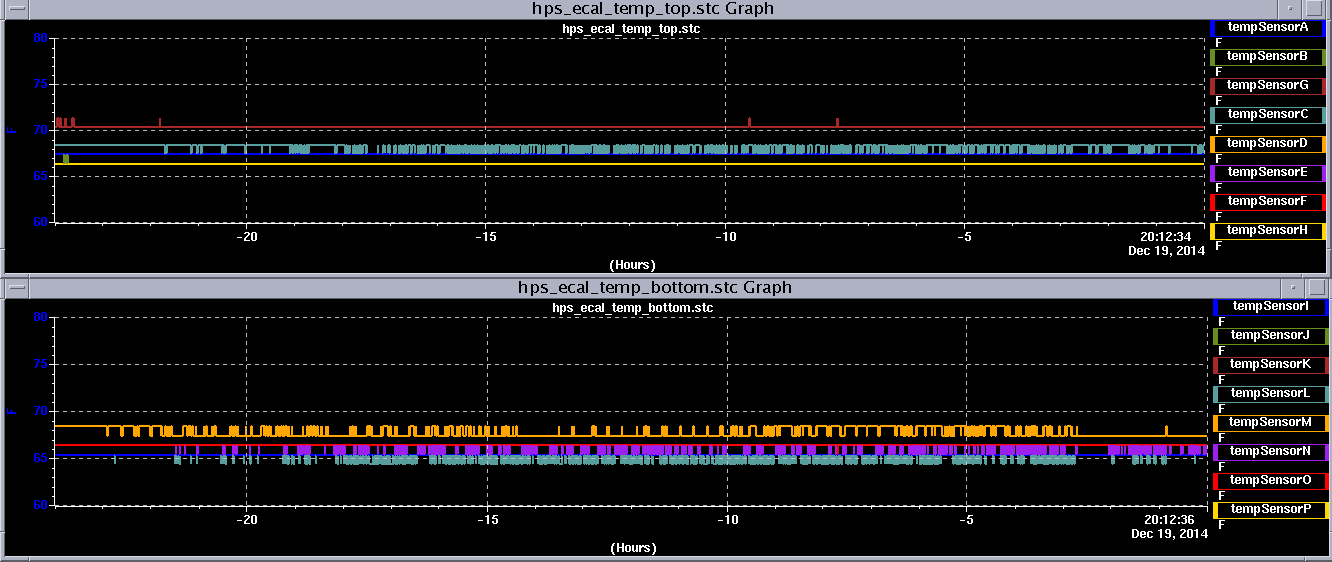
\includegraphics[width=0.45\textwidth,height=4.5cm]{pics/ECal_temp_s.png}
%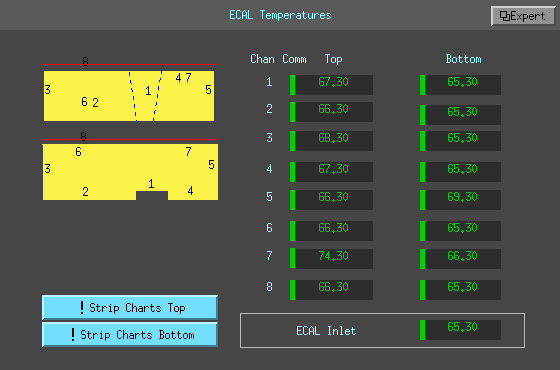
\includegraphics[width=0.39\textwidth]{pics/EcalTemp_2014_12_20.png}
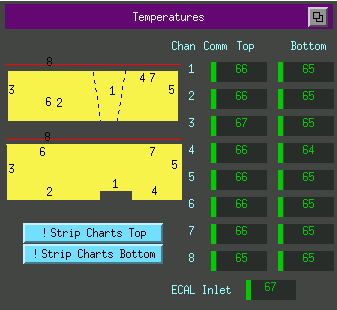
\includegraphics[width=0.3\textwidth,height=4.5cm]{pics/epics_ecal_temp.png}
\caption{\label{temp2} View of the EPICS temperature monitoring strip charts (left) and the temperature portion of the main RICH EPICS screen (right).}
\end{figure}

\subsection{Cooling System}
         The cooling allows to keep the calorimeter at the constant temperature and should be ON at all times. The cooling system can be monitored through its webcam and EPICS controls (figure~\ref{ChillerCam}). Shift takers should not attempt to change the cooling system settings and call RICH expert in case of problem.  The webcam is accessible in a web browser via the url \texttt{cctv10.jlab.org} and the ``Monitoring'' tab on the {\bf CLAS Run Wiki}.

\begin{figure}[htbp]
\center
%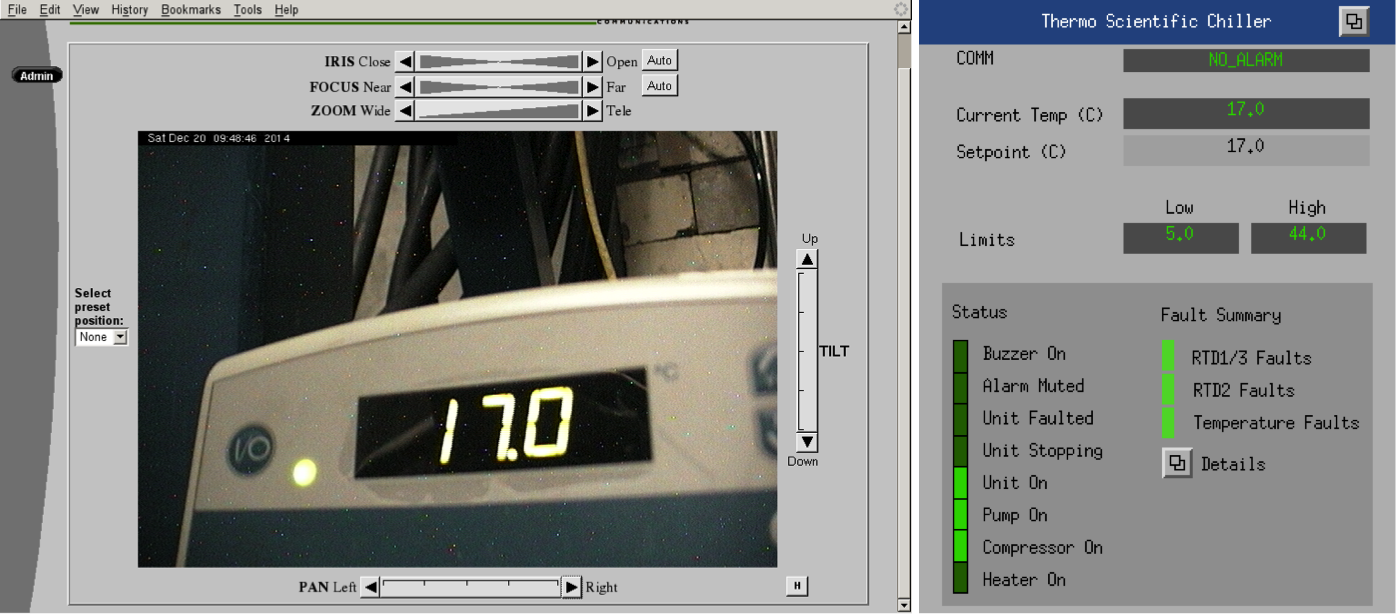
\includegraphics[width=0.99\textwidth]{pics/ChillerCombo.png}
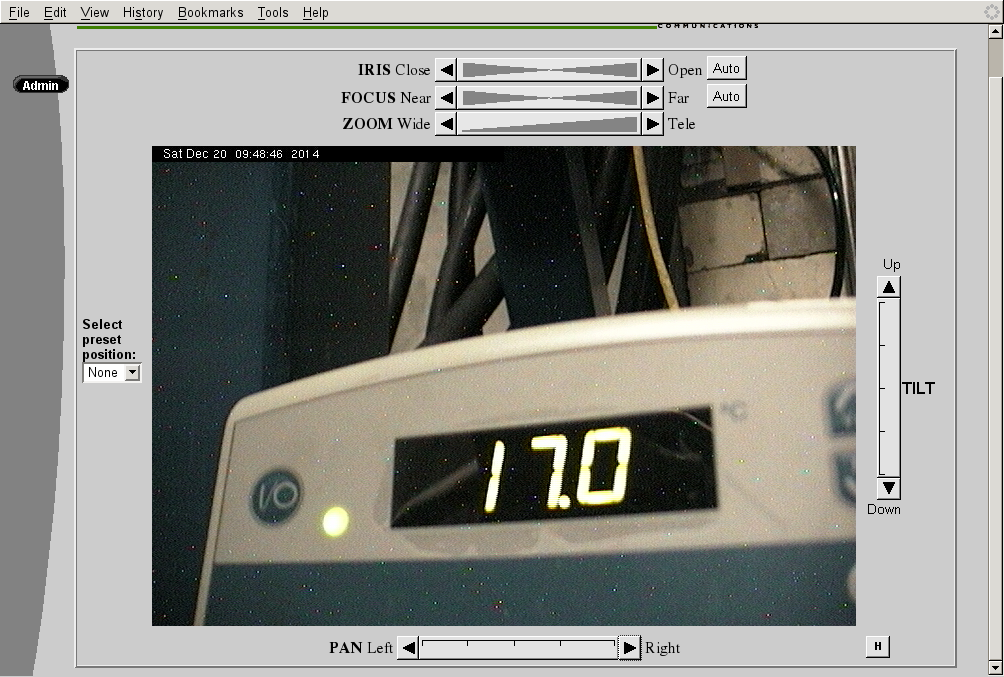
\includegraphics[width=0.45\textwidth,height=4.5cm]{pics/ChillerCam_2014_12_20.png}
%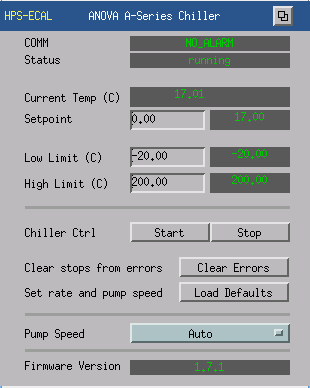
\includegraphics[width=0.3\textwidth,height=5.5cm]{pics/ChillerWin_2016_1_17.png}
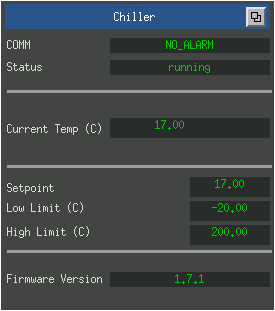
\includegraphics[width=0.3\textwidth,height=4.5cm]{pics/epics_ecal_chiller.png}
\caption{ \label{ChillerCam} View of the chiller's \texttt{cctv10.jlab.org} webcam (left) and its portion of the main RICH EPICS window (right).}
\end{figure}

%%%%%%%%%%%%%%%%%%%%%%%%%%%%%%%%%%%%%%%%%%%%%%%%%%%%%%%%%%%%%%%%%%%%%%
\newpage
{\color{blue}

\section{Low Voltage}
}
{\em The low voltage power supply must be on before HV is turned on, and changing its settings requires contact with an RICH-expert.}
      
LV should be monitored using its webcam and its portion of the main RICH EPICS screen (both shown in figure~\ref{LVCam}). Call the RICH expert if this appears not to be ON or shows an abnormal current for either of its two channels.  {\em Normal current is between 4.0 and 4.2 A for both channels}.  This webcam is accessible via the url \texttt{cctv11.jlab.org} in a web browser and the ``Monitoring'' tab on the main {\bf HPS Run Wiki}.
\begin{figure}[htbp]
\center
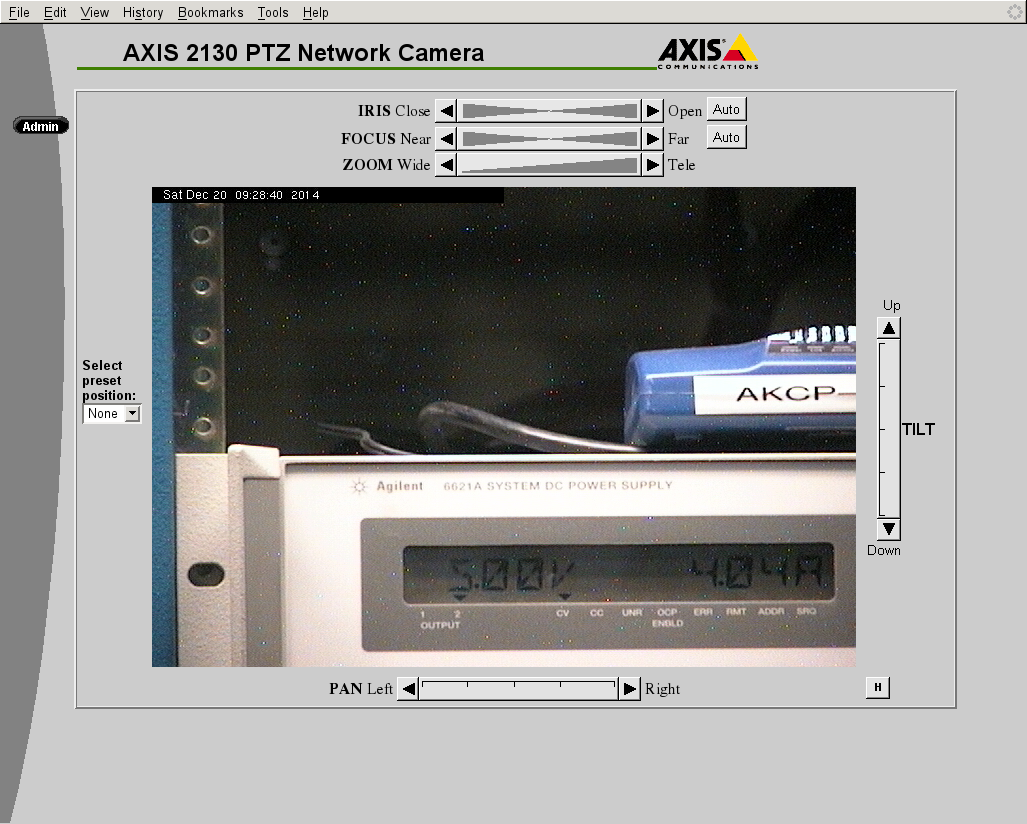
\includegraphics[width=0.49\textwidth,height=5.5cm]{pics/LVCam_2014_12_20.png}
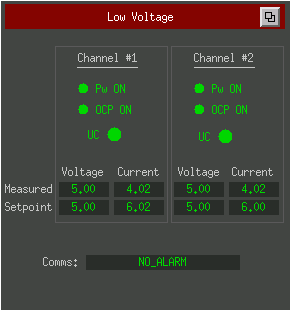
\includegraphics[width=0.39\textwidth,height=5.5cm]{pics/lvnovice.png}
\caption{ \label{LVCam} View of the LV suuply by webcam (\texttt{cctv11.jlab.org}) and its portion of the main RICH EPICS screen.}
\end{figure}

{\color{blue}

\section{High Voltage}
}
      \subsection{Turning ON/OFF High Voltages}

      The high voltage supply of the RICH is controlled and monitored using the main RICH
EPICS window (Figure ~\ref{fig:ecal_all}).  It has buttons to ramp up and down the entire 
calorimeter's high voltages (labeled {\bf ALL ON} and {\bf ALL OFF}), open windows for
individual channel control (figure~\ref{HVControl}), and open more detailed expert views 
(e.g. figure ~\ref{HV}).

   \subsection{HV Current Monitoring}
   Individual channels' currents can be monitoring in figure~\ref{HVControl}, and strip charts should be open for long term monitoring.  The strip charts are accessible from the main RICH screen (figure ~\ref{fig:ecal_all}) under the HV sections' {\bf Monitors} button (and also from the HPS\_EPICS screen (figure~\ref{EPICSmain}) via the {\bf Strip-Tool} button).  An example is shown in figure~\ref{fig:hvcurrentstrips}.  Jumps or drifts in current of more than 1 A should be noted in the logbook.

   \begin{figure}[htbp]\centering
       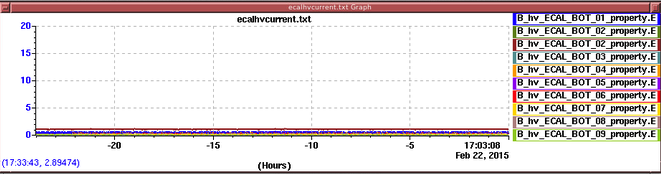
\includegraphics[width=16cm]{pics/hvcurrentstrip.png}
       \caption{HV Current strip charts.\label{fig:hvcurrentstrips}}
   \end{figure}


   \subsection{Responding to HV trips}

   HV problems, in particular trips, are indicated by a red group in the main RICH EPICS GUI (figure~\ref{fig:ecal_all}).  HV trips will also be announced by the alarm handler.  During normal operations with HV ON, there should be no red groups in Figure \ref{fig:ecal_all} and no RICH HV alarms.  In case of an HV trip, or a red region in Figure \ref{fig:ecal_all}:
\begin{itemize}
    \item Try to reenable the tripped HV group by turning it back on in the EPICS HV control screen (figure~\ref{HVControl}) accessed via the {\bf Controls} button in the main RICH EPICS screen (Figure \ref{fig:ecal_all}).  (An easier alternative is just pressing the {\bf ALL ON}
button in the main RICH EPICS screen.)
    \item Record the trip in the log book with precise indication of the group and run
        number concerned. 
\end{itemize}
Contact the RICH expert on-call in case of uncertainty.
      
      {\em Note, the HV can take up to 3 minutes to turn back on so you should end the current run and begin a new one when the high voltage is back on. If you cannot get a HV group to work contact the RICH expert on call.}

      {\bf If you encounter more than two HV trips during your shift for the same group, you should notify the RICH Expert.}

\begin{figure}[htbp]
\center
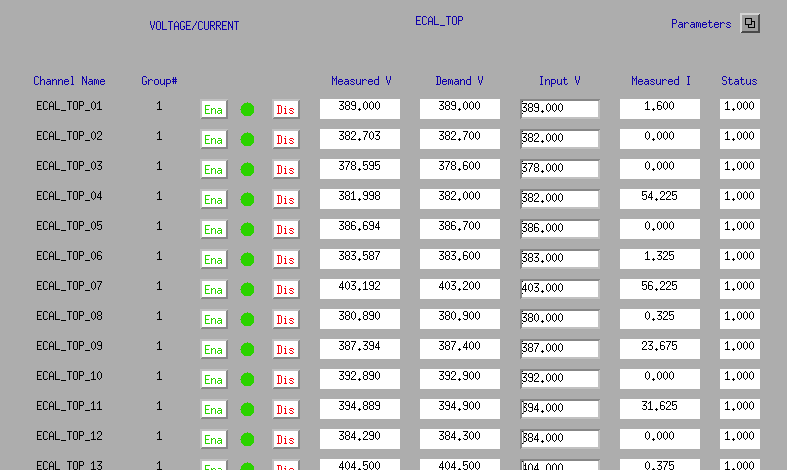
\includegraphics[width=0.85\textwidth]{pics/ecalhv_setting_2014_12_15-SUBSET.png}
\caption{ \label{HVControl} Cropped view of the EPICS RICH HV control window for individual channels.}
\end{figure}

\clearpage
{\color{blue}

\newpage
      \section{Scalers}
}
      Rates seen by the RICH are available in the ROOT-based GUI shown in Figure \ref{Scalers}, which represent the rates as seen by the RICH electronics.  This display is accessible via the main CLAS\_EPICS window under the {\bf RICH Scaler GUIs} button, and also by running the command \texttt{clas\_rich\_scalers} in a terminal. 
 
 %     One can also see clustering scalers from the DAQ ``diaggui'' screen (figure~\ref{DAQscalers}), accessible also by the {\bf RICH Scaler GUIs} button or by executing \texttt{diaggui.sh} in a terminal.  This GUI indicates the rates of clusters reconstructed by the trigger electronics. 
      
      These numbers should all remain constant within $^\sim10\%$ during stable beam operation. A strong increase is the indication of bad beam conditions or the presence of a new source of noise in the RICH system.  If the latter case, please contact RICH expert on call.
\begin{figure}[htbp]
\center
%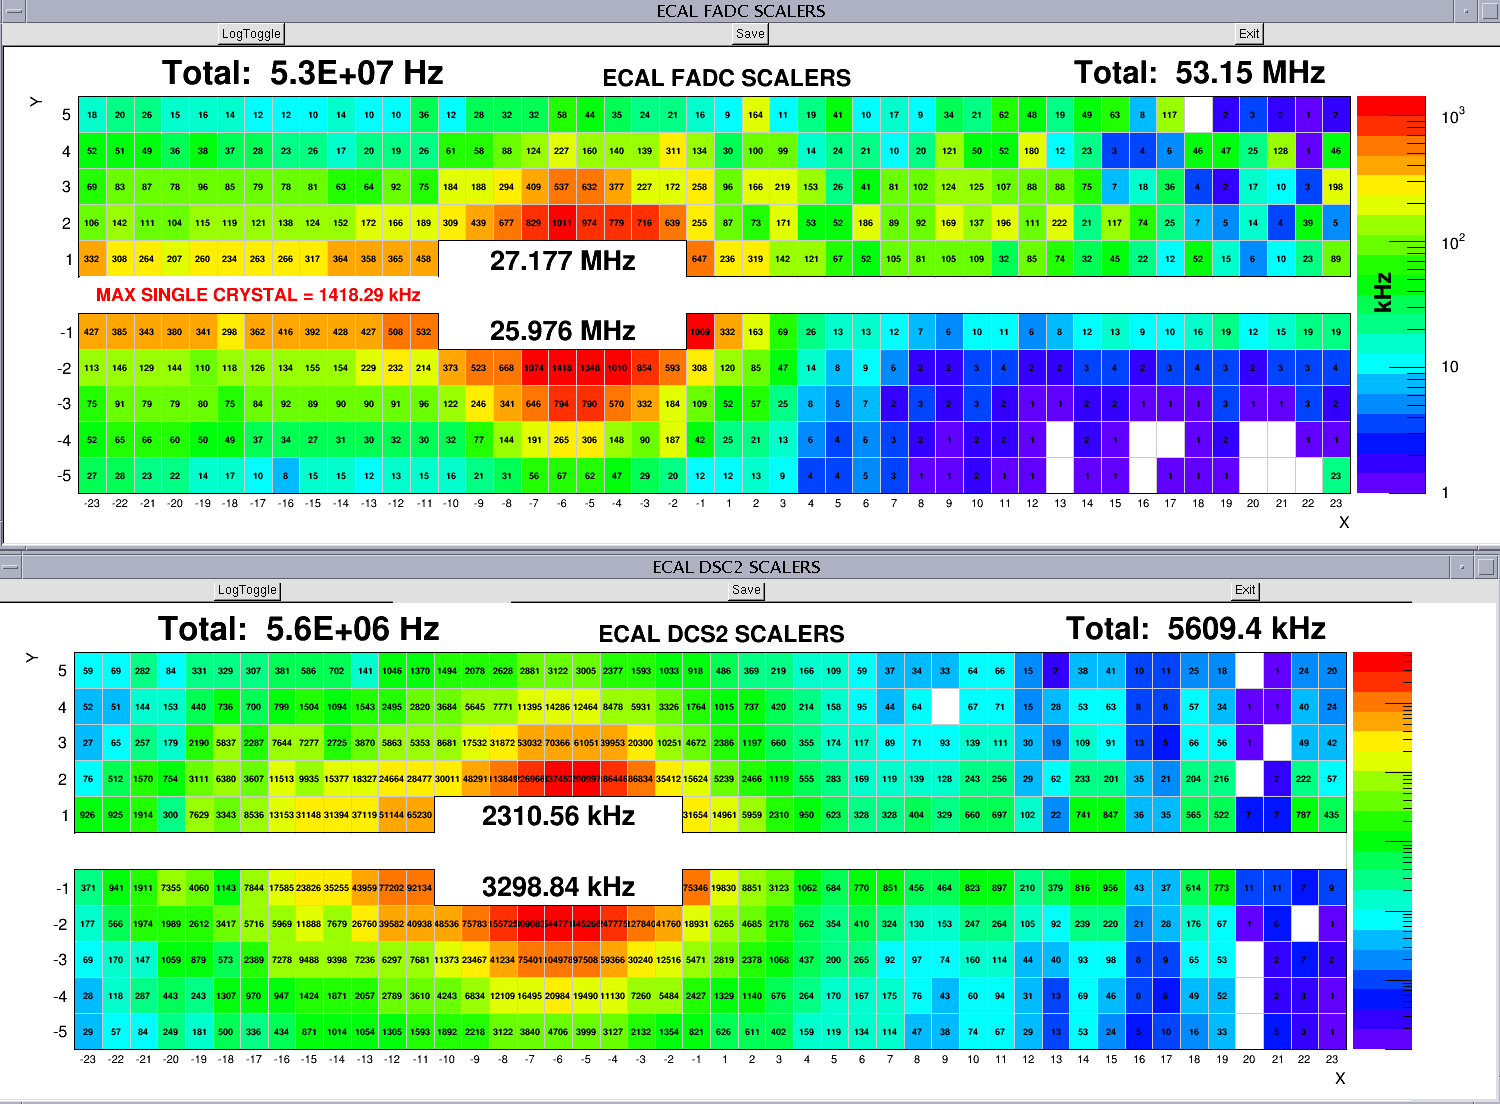
\includegraphics[width=0.75\textwidth]{pics/ECAL_FADC_SCALER_2014_12_20.png}
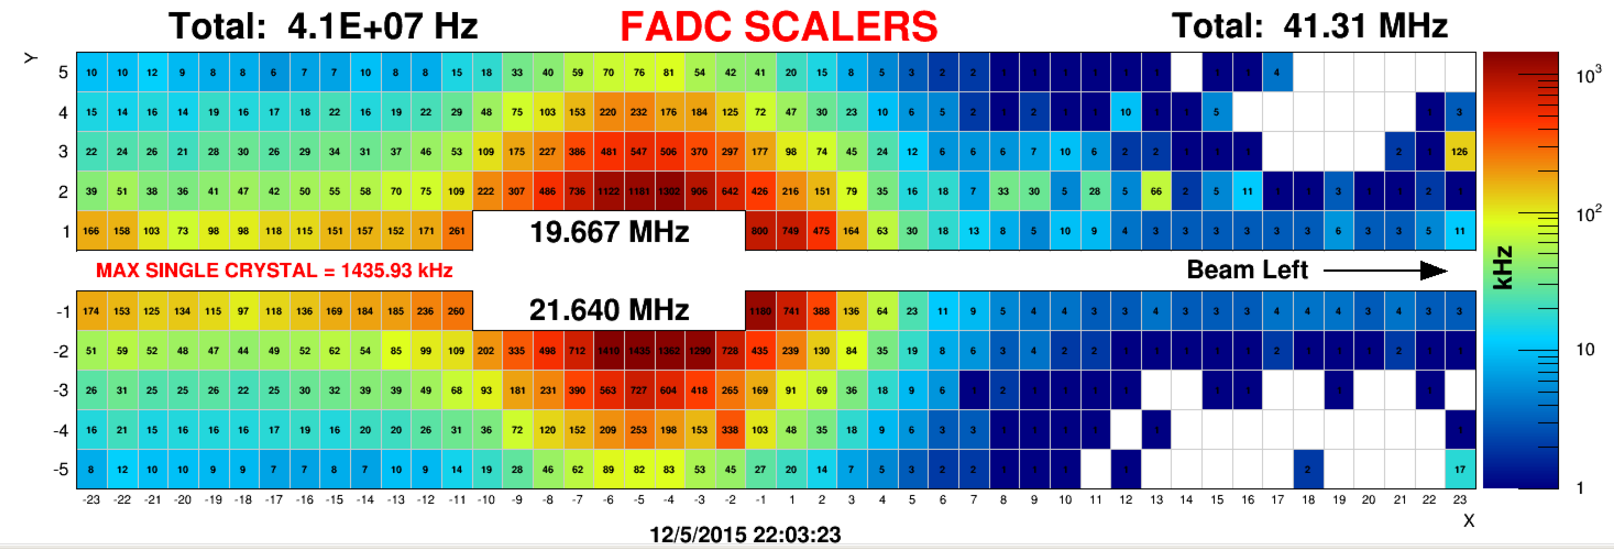
\includegraphics[width=0.9\textwidth]{pics/fadcscalers_2015run.png}
\caption{ \label{Scalers} View of the EPICS RICH scalers window.}
\end{figure}
%\begin{figure}[htbp]
%\center
%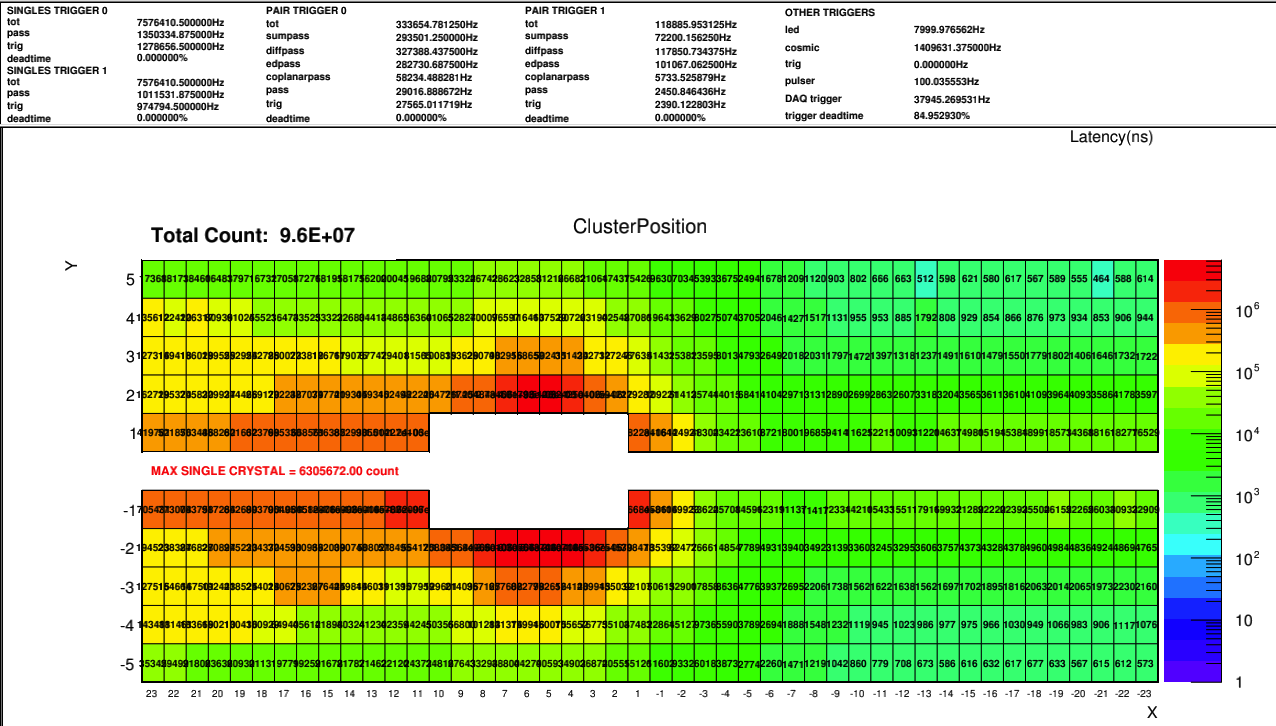
\includegraphics[width=0.9\textwidth]{pics/ecal-cluster-12-20-14.png}
%\caption{ \label{DAQscalers} View of the DAQ scaler window.}
%\end{figure}
{\color{blue}
\newpage
  \section{Strip Charts}
  }
      The most import quantities to monitor with strip charts are temperature and HV current.  
%There are two programs to view strip charts of RICH EPICS variables.  The older StripTool shown in figure~\ref{temp2} can be started from the HPS\_EPICS gui.
  The MyaViewer (which adds the ability to retrieve archive information) can be run by executing the following scripts in a terminal:
      
      \begin{itemize}
          \item \texttt{mya\_rich\_all.sh}
          \item \texttt{mya\_richl\_temp.sh}
          \item \texttt{mya\_rich\_curr.sh}
          \item \texttt{mya\_rich\_voltage.sh}
      \end{itemize}
{\color{blue}
\section{Monitoring App}
}
The hps-java monitoring app is used to run full calorimeter reconstruction on live events from the daq on the ET ring.  It provides many plots to assess detector performance.  To start the monitoring app, in a terminal run:
\begin{center}\texttt{startRICHMonitoring}\end{center}
Then click the ``connect'' button to connect to the ET ring.

At the start of every run, the monitoring app should be disconnected and reconnected to the ET ring.  After a few minutes of beam, the tabs should be cycled through and their plots compared to the reference.  Once sufficient statistics are accumulated, the plots should be saved as a pdf and uploaded to the logbook.

\newpage
%%%%%%%%%%%%%%%%%%%%%%%%%%%%%%%%%%%%%%%%%%%%%%%%%%%%%%%%%%%%%%%%%%%%%%
%%%%%%%%%%%%%%%%%%%%%%%%%%%%%%%%%%%%%%%%%%%%%%%%%%%%%%%%%%%%%%%%%%%%%%
%%%%%%%%%%%%%%%%%%%%%%%%%%%%%%%%%%%%%%%%%%%%%%%%%%%%%%%%%%%%%%%%%%%%%%
%%%%%%%%%%%%%%%%%%%%%%%%%%%%%%%%%%%%%%%%%%%%%%%%%%%%%%%%%%%%%%%%%%%%%%
%%%%%%%%%%%%%%%%%%%%%%%%%%%%%%%%%%%%%%%%%%%%%%%%%%%%%%%%%%%%%%%%%%%%%%
%%%%%%%%%%%%%%%%%%%%%%%%%%%%%%%%%%%%%%%%%%%%%%%%%%%%%%%%%%%%%%%%%%%%%%
\iffalse
   \section{LED Monitoring}
      \subsection{System operations}
      The LED system is operated through an EPICS GUI accessible from the main HPS EPICS menu, through Devices, then Flasher (see Figure \ref{FlasherMEDM}).

Shift takers are requested to operate the system in ``Sequence mode'' only. To do so, when requested, click on ``Initialize Flasher'', then verify the TOP frequency is 8000 Hz, and if necessary adjust it trough the proper drop-down menu. Finally, to start the sequence, click on ``Start Blue Seq'' (to use blue LEDs) or ``Start Red Seq'' (to use red LEDs). During such a run the DSC scaler screen allows to check the proper functioning of the channels (figure~\ref{LEDScalers}). 

\begin{figure}[htbp]
\center
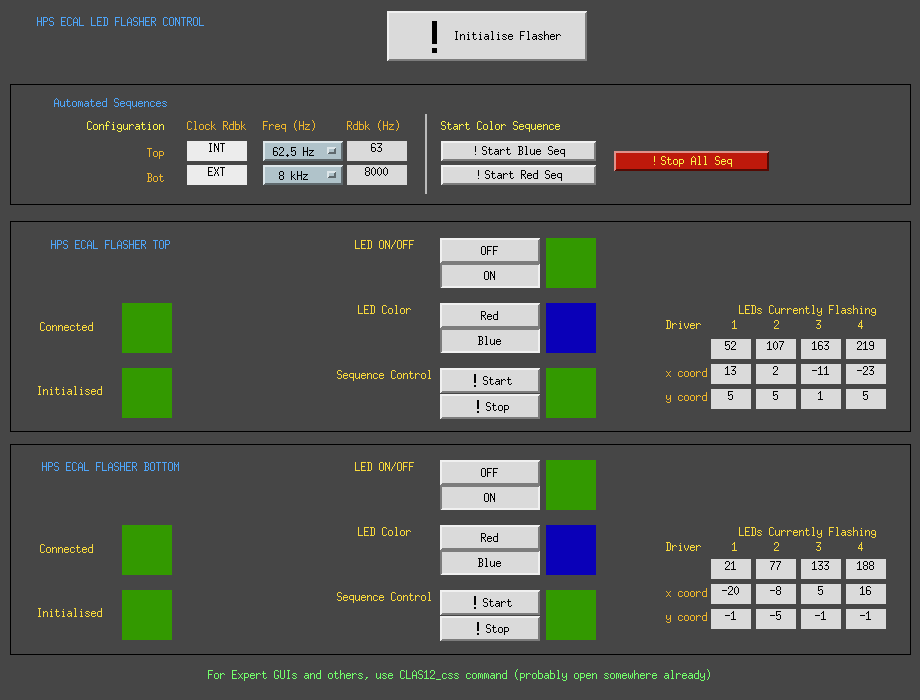
\includegraphics[width=0.75\textwidth]{pics/FlasherMEDM.png}
\caption{ \label{FlasherMEDM} The HPS-ECAL Led monitoring system EPICS GUI.}
\end{figure}
\begin{figure}[htbp]
\center
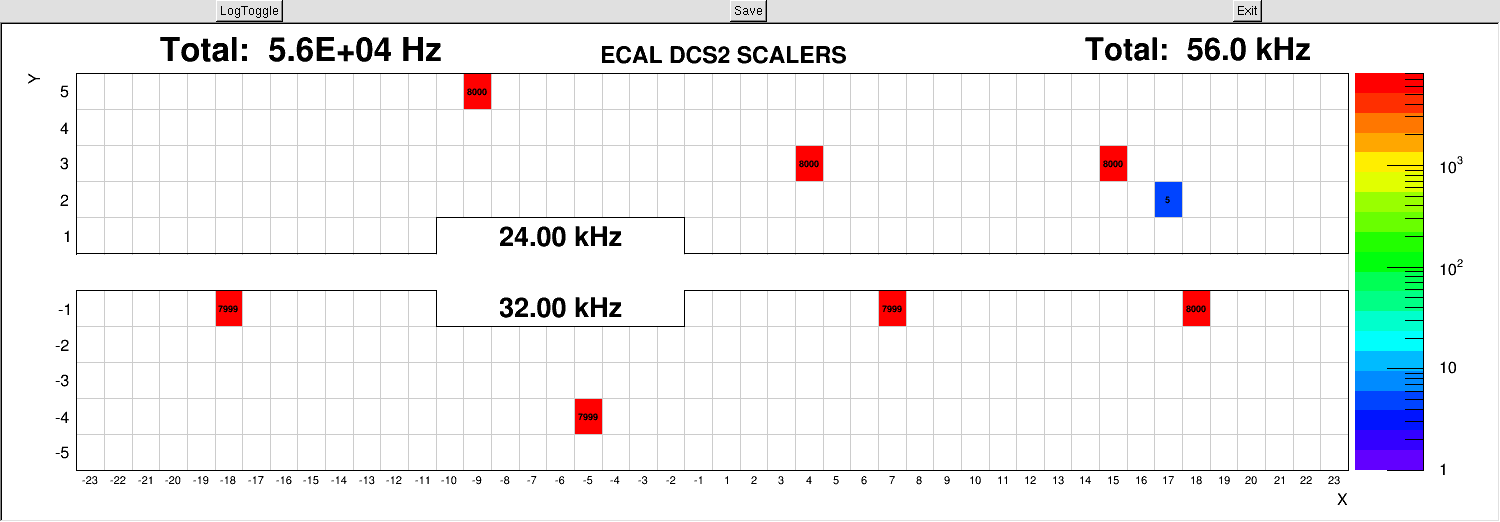
\includegraphics[width=0.95\textwidth]{pics/DSCScalersLED_2014_12_20.png}
\caption{ \label{LEDScalers} The HPS DSC scaler during a LED run.}
\end{figure}

\subsection{Automatic LED Monitoring}
A monitoring app is setup to record all channels successfully registered during an LED run.  It should be started before the LED sequence is started and viewed afterwards, with the command: \begin{center}\texttt{\$HOME/hps\_software/scripts/startECalLEDSequenceMonitoring.csh}\end{center} Make sure to use the hpsrun account before using this command.
  
\subsection{Taking an LED sequence run}
The following instructions must be followed to take an LED sequence run. This involves setting the DAQ, starting the LED sequence run, and configure the hps-java monitoring app to monitor the data. At the end of the run, the user can upload the relevant information to the hps conditions database, as well as post a log-entry to the HallB electronic logbook.

\subsubsection{Setup}
Follow these instructions to setup the system before takin the LED sequence run.
It is critical they are followed in the \textbf{exact} order as they are here reporter.

\begin{enumerate}
\item{\textbf{Start the DAQ system: }
\begin{itemize}
\item Identify the machine where the DAQ RunControl is running. If you can't find it anywhere, it is possible the DAQ system has to be initialized from scratch. To do so, refer to the HPS DAQ manual, or contact the DAQ expert.
\item Depending on the DAQ state, different buttons may be visible in the ``Transition'' area. If the ``Configure'' button is not visible, click on ``Reset'', then on ``OK''.
\item Click on ``Configure'' to properly set up the run.
A ``Run Type Configuration'' dialog will show up.

Use the scroll-down menu to select as RunType: HPS35\_ECAL. This configuration will also save any data on tape (online analysis will be performed).

Use instead: HPS35\_ECAL\_NOER to not save data on tape.

\textit{Default is to save data to the tape}
\item{Click on ``Download'' button. A file-chooser menu will show up.

Select: HPS $\rightarrow$ ECAL $\rightarrow$  HPS\_ECAL\_LED\_RUN.trg. 

Click on ``OK'' to close the file-choose menu.
}
\item{Click on ``Prestart''.  Wait until the ``GO'' button appears, but {\bf do not click on it yet.}

 }
\end{itemize}
}
\item{\textbf{Start the monitoring app: }Use the command outlined in the previous section to start the monitoring app.

\textcolor{red}{\bf Do this after the run-control shows the ``GO'' button.}

When the main gui window shows up, click on the ``Connect button''. The Ecal event display will show up.}
\item{\textbf{Initialize the LED monitoring sequence:}In the EPICS gui, click on ``Initialise Flasher'', then on ``!Stop All Seq'' (to ensure there are no previous sequences running). 

For both controllers, ensure the LED ON/OFF button is set to OFF (RED square). If not, click on OFF.}
\end{enumerate}
      
\subsubsection{Run start, data taking, and run stop}
To start data taking follow these instructions, in the exact order they are reported here.
\begin{enumerate}
\item In the RunControl GUI, click on the ``GO'' button. Wait 10~s, until the message ``transiction go succeded'' is displayed in the log window and the ``END'' button displays. 
\item In the EPICS gui, click on ``Start Blue Seq'' or ``Start Red Seq''.

By default, take a BLUE sequence. 

Take a RED sequence only if the Ecal expert ask you to do so.
\end{enumerate}

While the LED sequence is running, you can look at the monitoring application to check data being recorded. The event display will show 8 crystals at time with a signal. A full sequence will take $\simeq$ 10 minutes to complete.

{\bf  The DAQ system is not set up to end the run when the LED sequence is completed.} When the sequence is complete:
\begin{itemize}
\item The LED system automatically turns off. As a direct consequence of this, no further triggers are sent to the DAQ system
\item The data-taking run is \textbf{not} ended. This means the DAQ will stay in RUN mode, but no events will be recorded, since there are no triggers.
\end{itemize}
{\bf
Use the EPICS gui to periodically check the sequence status, looking at the Sequence Control section (RED is OFF, GREEN is ON). Tipically, a sequence will take $\simeq$ 10 minutes to complete.}

The user can confirm the sequence has actually ended by looking at the ECal Event display: no crystals have signal when the sequence is off.

When both sequences are OFF, first turn OFF both controllers (LED ON/OFF, click on OFF), 
then use the DAQ run control to END the run, by clicking on the ``End'' button.



\subsubsection{Analysis at the run end}

When the run ends, the monitoring application automatically recognizes this, and the online analysis of the measured data starts. 

A pop-up will appear, asking the user if he wants to upload the LED data that has been measured to the HPS conditions database: uploaded quantities are the average channel response to LED pulses and the RMS. Before confirming this, the user is required to have a look at the average charge per LED, displayed in the monitoring app: tab Ecal Led Sequence, sub-tab Sequence Map. The average channel response should be in the range $\simeq 20 \div 30$. 

An automatic log entry in the Hall B logbook will also be made, with the Sequence Map image. The user is requested to complete the comment form with any relevant observation, and then click on ``OK''

{\bf {\it TODO: print a reference map and aks the user to compare with that}}

\subsection{Quick 2-Minute LED Run for Simple Channel Status Check}
{\em Note, this has become deprecated and unsupported now that we replaced splitters with
patch panels and no longer have discriminators.  Using FADCs to perform the same task is
possible but yet to be implement, since that requires reconfiguring the FADC boards'
thresholds every time and lessens the quickness and usefulness of this.}

This just counts threshold crossings in the discriminators, which is sufficient for checking that all channels are alive with LEDs.  This full test of all 442 channels requires only 2 minutes, requires no changes to the DAQ configuration, and is completetely independent of the hps-java monitoring app.  If all LEDs and all channels are working, the result should be similar to Figure~\ref{fig:quickledscanresult}

  \begin{enumerate}
      \item With a quiet detector, execute the command \texttt{runEcalLedTest.sh}.  This will open a gui showing accumulated scaler rates in all 442 ECal channels.  
      \item Start a ``LessFast'' LED sequence.
      \item Check that all channels are uniformly populated to within a factor of 2 after the sequence is finished.
  \end{enumerate}

  \begin{figure}[htbp]\centering
      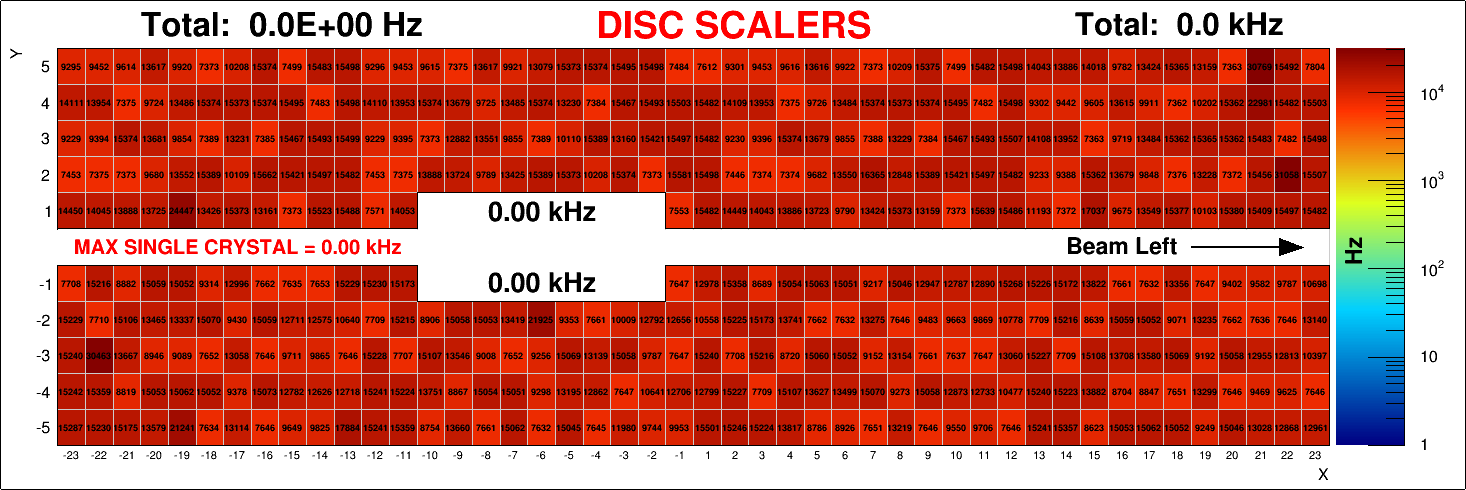
\includegraphics[width=14cm]{pics/ledScanBlue_2015_04_17_10-45-53.png}
      \caption{The accumulated discriminator counts after a successfull ``Quick 2-Minute LED Run''.  The absolulte counts will depend on LED pulser rate and duration, but the important aspect is uniformity from channel to channel.  \label{fig:quickledscanresult}}
  \end{figure}


   \section{Taking a Cosmic Calibration Run}

   In addition to the calorimeter's HV, the cosmic PMTs should also be powered on.  Their HV control is under {\bf Cosmic PMTs} in the {\bf Controls} button of the main ECal EPICS screen's HV section (Figure ~\ref{fig:ecal_all}) and shown in Figure~\ref{fig:cosmicPMTs}.  They are named \texttt{ECal\_cosm1} and \texttt{ECal\_cosm2} and their voltages should be set at 1650 V.  The DAQ configuration should be set to \begin{center}\texttt{hps\_cosmic.trg}\end{center} and a normal cosmic trigger rate is about 5 Hz.
       \begin{figure}[htbp]\centering
           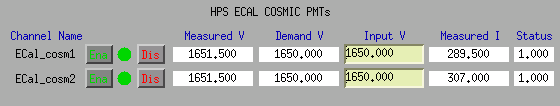
\includegraphics[width=0.8\textwidth]{pics/cosmicPMTs.png}
           \caption{Controls for PMTs for cosmic trigger.\label{fig:cosmicPMTs}}
       \end{figure}


   \section{Taking a Pedestal Run}

   \subsection{With Beam}
   Pedestals are calculated at running luminosity with DAQ configuration \begin{center}\texttt{ecalPedestal.trg}\end{center} and monitored and analyzed with HPS's hps-java monitoring app via the command:
       \begin{center}\texttt{startEcalPedestalCalculator}\end{center}
       In this monitoring app you can click on the event display to view the different channels' pedestal histograms as the data is acquired.  Once the statistics are sufficient, the app should be disconnected from the ET-ring and then output files for the DAQ and database will be generated in the directory:\begin{center}\texttt{\$HOME/EcalPedestals}\end{center}  The user will be asked if they want them put in the database automatically, and it requires two consecutive ``YES'' responses to make it happen.  An expert should make the trigger configuration use the new pedestal file.

         \subsubsection{Installing the new pedestals}
      To generate the pedestal file for the DAQ, run this script, where the last argument is the name of the file generated in the previous step:
         \begin{center}\texttt{calibUtilHpsEcal.py -P -DAQ -N -b XYZ\_hpsDB.txt}\end{center}

  \subsection{Without Beam}
  Coming soon.

    \section{Taking a FEE Run for Gain Calibration}
Use the trigger file
\begin{center}\texttt{HPS/Run2016/fee\_200nA.trg}\end{center}
  The trigger rate should be about 30 kHz for 200 nA beam.  Along with the standard ECal monitoring app, there is a special one for FEE monitoing which allows to see the FEE spectra for each channel:
\begin{center}\texttt{startEcalFeeData}\end{center}

\fi
%%%%%%%%%%%%%%%%%%%%%%%%%%%%%%%%%%%%%%%%%%%%%%%%%%%%%%%%%%%%%%%%%%%%%%
%%%%%%%%%%%%%%%%%%%%%%%%%%%%%%%%%%%%%%%%%%%%%%%%%%%%%%%%%%%%%%%%%%%%%%
%%%%%%%%%%%%%%%%%%%%%%%%%%%%%%%%%%%%%%%%%%%%%%%%%%%%%%%%%%%%%%%%%%%%%%
%%%%%%%%%%%%%%%%%%%%%%%%%%%%%%%%%%%%%%%%%%%%%%%%%%%%%%%%%%%%%%%%%%%%%%
%%%%%%%%%%%%%%%%%%%%%%%%%%%%%%%%%%%%%%%%%%%%%%%%%%%%%%%%%%%%%%%%%%%%%%
%%%%%%%%%%%%%%%%%%%%%%%%%%%%%%%%%%%%%%%%%%%%%%%%%%%%%%%%%%%%%%%%%%%%%%


\newpage

\part{RICH Experts Resources}
%
%{\color{blue}
%   \section{Location of RICH Elements}
%}
%   {\em{\bf REMINDER:} Since the ECal is within 3 feet of the beamline, it needs to be surveyed by RADCON before any work can be done on it.}
%   {\footnotesize
%\begin{itemize}
%\item
%The chiller is located beam-left just downstream of the calorimeter on the ground in the Alcove.
%\item
%The LED controllers are located at the top of the rack closest to the beamline in the Alcove.
%\item
%The TDCs and DISCs are are in the rack closest to the beamline in the Alcove.
%\item
%The FADCs and patch panels occupy the rack furthest from the beamline in the Alcove.
%\item
%    The HV supply is on the Pie Tower in the rack closest to the beamline.  See figure~\ref{fig:HVPHOTO}.
%\item
%    The LV supply is on the Pie Tower at the top of the middle rack. See figure~\ref{fig:LVPHOTO}.
%\end{itemize}
%}
%\begin{figure}[htbp]\centering
%    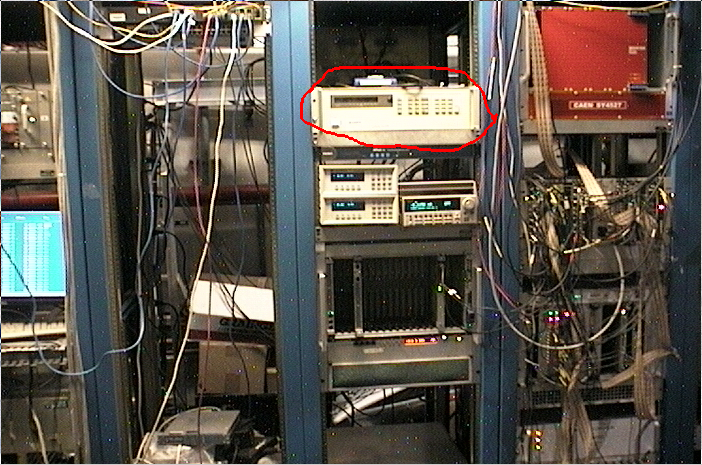
\includegraphics[width=7cm]{pics/ECALLVPHOTO2.png}
%    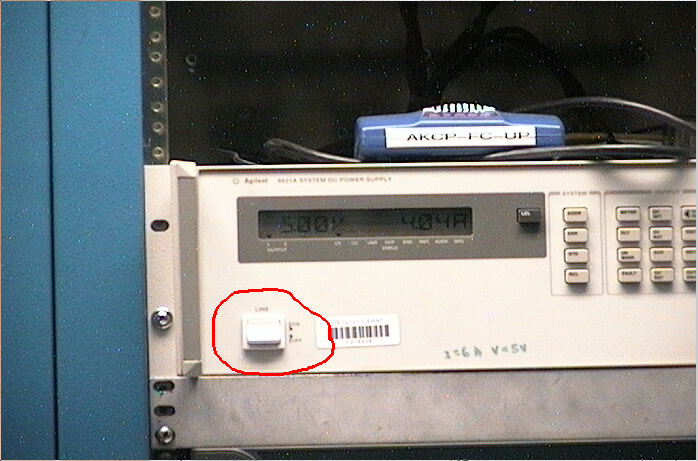
\includegraphics[width=7cm]{pics/ECALLVPHOTO.png}
%    \caption{Location of Agilent LV power supply near the top of the middle rack in the pie tower.  Power switch is circled in red.\label{fig:LVPHOTO}}
%\end{figure}
%\begin{figure}[htbp]\centering
%    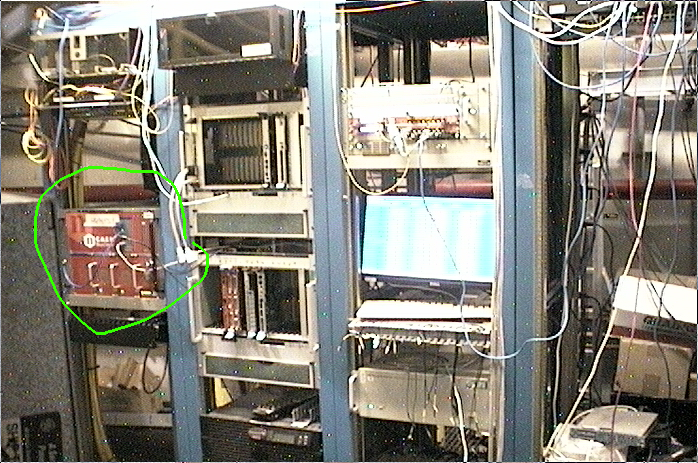
\includegraphics[width=9cm]{pics/ECALHVPHOTO.png}
%    \caption{Location of the CAEN SY4527 HV power supply in the left-most rack in the pie tower.  Key for on/off is in the lower right corner of the crate.  The crate is labeled ``HVHPS2''. (The LV supply is just out of the picture to the right.)\label{fig:HVPHOTO}}
%\end{figure}

%\newpage
{\color{blue}
   \section{Cooling system}
}
High capacity air compressors supply clean dry air at room temperature to cool the electronics package inside the detector. The plan is to have 2 compressors in parallel charging a 1000 liter capacity air tank. Air pressure is reduced to supply manual valve flow meters, one per detector. In the case of a power outage, the air tank should contain sufficient air to remove the latent heat of the electronics package.

Powering up the electronics package inside the RICH without cooling may result in severe damage or fire. Interlocking RICH HV and LV power supply operation to proper cooling circuit operation eliminates this hazard.
The interlocks perform two functions in the case of a cooling system fault
\begin{itemize}
\item Turn off power to the electronics package.
\item  Prevent energizing the electronics package.
\end{itemize}
There are 3 cooling circuit interlocks.
\begin{itemize}
\item Air Compressor Operation: minimum one compressor operating.
\item Minimum Air Pressure in Tank.  
\item Minimum Cooling Air Flow.
\end{itemize}
All three interlocks must be true in order for the electronics package to have power.

   The cooling system can be controlled through EPICS (\ref{ChillerCam}). 

     \subsection{Rebooting the Cooler system After Power Failure}

     If the cooler system  loses power while in local mode, the ``power'' button must be pressed manually to restart it after power is restored.  In case it loses power while in remote mode, a procedure is necessary to reset it after power is restored:
   {\footnotesize
     \begin{enumerate}
         \item Hold the ``up'' and ``down'' arrow buttons simultaneously for 10 seconds.
         \item Press the ``computer'' button to go into local mode.
         \item Press the ``power'' button to turn it off.
         \item Press the ``power'' button to turn it on.
         \item Press the ``computer'' button to return to remote mode.
    \end{enumerate}
    }

    \subsection{Restarting the Cooler System IOC}
    Chiller IOC runs in ``procserv'', a wrapper that automatically runs and restarts services and provides access to them via telnet.  To restart the chiller's IOC:
   {\footnotesize
   \begin{enumerate}
       \item \texttt{`softioc\_console iocchiller'} and type user's password if necessary.
       \item \texttt{`ctrl-x'} to restart the IOC
       \item \texttt{`ctrl-]'} to quit to telnet
       \item \texttt{`quit'} to exit telnet
   \end{enumerate}
   }
\noindent{\em Don't leave a terminal open connected to this telnet session.}

   \subsection{Restarting the Temperature Monitoring IOC}
   Thermocouples are used to monitor the temperature inside and outside the calorimeter.  To restart the IOC that reads these:
   {\footnotesize
   \begin{enumerate}
       %\item \texttt{`ssh hpsrun@clonsl1'}
       \item \texttt{`softioc\_console ioctempSens'} and type user's password if necessary.
       \item \texttt{`ctrl-x'} to restart the IOC
       \item \texttt{`ctrl-]'} to quit to telnet
       \item \texttt{`quit'} to exit telnet
   \end{enumerate}
   }
\noindent{\em Don't leave a terminal open connected to this telnet session.}


\newpage
{\color{blue}
   \section{LV Supply}
   }
      The low voltage power supply is an Agilent 6621.  It should be set with both channels at $+5$V with their current limits at 6 A, while external wiring inverts one channel to create a bipolar $\pm5$V supply. 

      The low voltage supply might have difficulties to get to full voltage because of high current. If that was the case check, with all power supplies off, that all connection are goods. Then contact run coordinator to see if LV power supply addition is possible. 

\subsection{Changing LV Settings}
The LV supply can be controlled via its EPICS expert screen (figure~\ref{lvexpert}), accessible from the grey button in the top right of the LV section of the main ECAL EPICS screen (figure~\ref{fig:ecal_all}). In general the only necessary changes are powering on/off, while voltage and current setpoints are never changed from 5V/6A.
\begin{figure}[htbp]\centering
    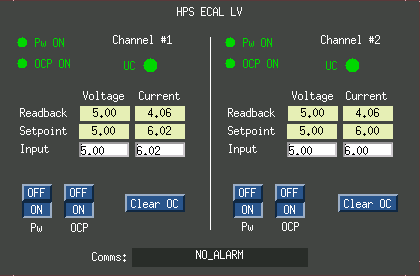
\includegraphics[width=9cm]{pics/lvexpert}
    \caption{The LV expert EPICS screen in normal operation.\label{lvexpert}}
\end{figure}

{\em Note, as a safeguard, if one currently tries to use EPICS to set the voltage greater than 5 V or the current greater than 6 A, the request will be ignored by the IOC.}  Overriding these limits can currently only be done either via local control (Section \ref{sec:lvlocalops}), or by setting new values for the limits via \texttt{caput}.  The corresponding PVs are:
{\footnotesize
\begin{itemize}
    \item\texttt{HPSECALLV:i1set:DRVH}
    \item\texttt{HPSECALLV:i2set:DRVH}
    \item\texttt{HPSECALLV:v1set:DRVH}
    \item\texttt{HPSECALLV:v2set:DRVH}
\end{itemize}
}
\subsubsection{Local Operation}\label{sec:lvlocalops}
The LV supply can also be controlled manually in the hall via buttons on its front panel.  However, when in remote mode (denoted by the ``RMT'' marker in its LCD display), local operations require pressing the ``LCL'' button first, then quickly pressing the desired operation button before remote mode is automatically reenabled by the IOC.  Completely disabling this ``feature'' requires stopping the IOC (see section~\ref{lviocstop}).

\subsection{Restarting the LV IOC}
   To restart the IOC:
   {\footnotesize
   \begin{enumerate}
       %\item \texttt{`ssh hpsrun@clonsl1'}
       \item \texttt{`softioc\_console iocA6621'} and type user's password if necessary.
       \item \texttt{`ctrl-x'} to restart the IOC
       \item \texttt{`ctrl-]'} to quit to telnet
       \item \texttt{`quit'} to exit telnet
   \end{enumerate}
   }
\noindent{\em Don't leave a terminal open connected to this telnet session.}

\subsection{Disabling the LV IOC}\label{lviocstop}
   To disable the IOC:
   {\footnotesize
   \begin{enumerate}
       %\item \texttt{`ssh hpsrun@clonsl1'}
       \item \texttt{`softioc\_console iocA6621'} and type user's password if necessary.
       \item \texttt{`ctrl-t'} to toggle auto-restart
       \item \texttt{`ctrl-x'} to kill the IOC
       \item \texttt{`ctrl-]'} to quit to telnet
       \item \texttt{`quit'} to exit telnet
   \end{enumerate}
   }
\noindent{\em Don't leave a terminal open connected to this telnet session.}

\newpage
{\color{blue}
   \section{High Voltage}
   }
   \subsection{Restarting the HV IOC}
   Occaissonaly the soft IOC for the HV needs to be manually restarted.  Symptoms of this condition include errors messages from EPICS when trying to turn on/off voltages and white blocks in the main HV screen (figure~\ref{HV}).  
   
   To restart the IOC:
   {\footnotesize
   \begin{enumerate}
       %\item \texttt{`ssh hpsrun@clonsl1'}
       \item \texttt{`softioc\_console iocecalVoltages'} and type user's password if necessary.
       \item \texttt{`ctrl-x'} to restart the IOC
       \item \texttt{`ctrl-]'} to quit to telnet
       \item \texttt{`quit'} to exit telnet
   \end{enumerate}
   }
\noindent{\em Don't leave a terminal open connected to this telnet session.}

{\bf\em Note, this IOC always needs to be restarted if the HV CAEN mainframe is power cycled.}
   
   \subsection{Changing HV Settings}
      {\bf NOTE:} Changing voltage settings should be taken care of in coordination with the RICH group. 

 {\bf NOTE:} The RICH HV groups were renumbered for EPICS, and the correspondence map 
 %(figure~\ref{ExpertMap}) 
 will be available in the expert RICH HV monitoring window (Figure 
 \ref{HV}) via the ``Expert HV Map'' button.

\begin{figure}[htbp]
\center
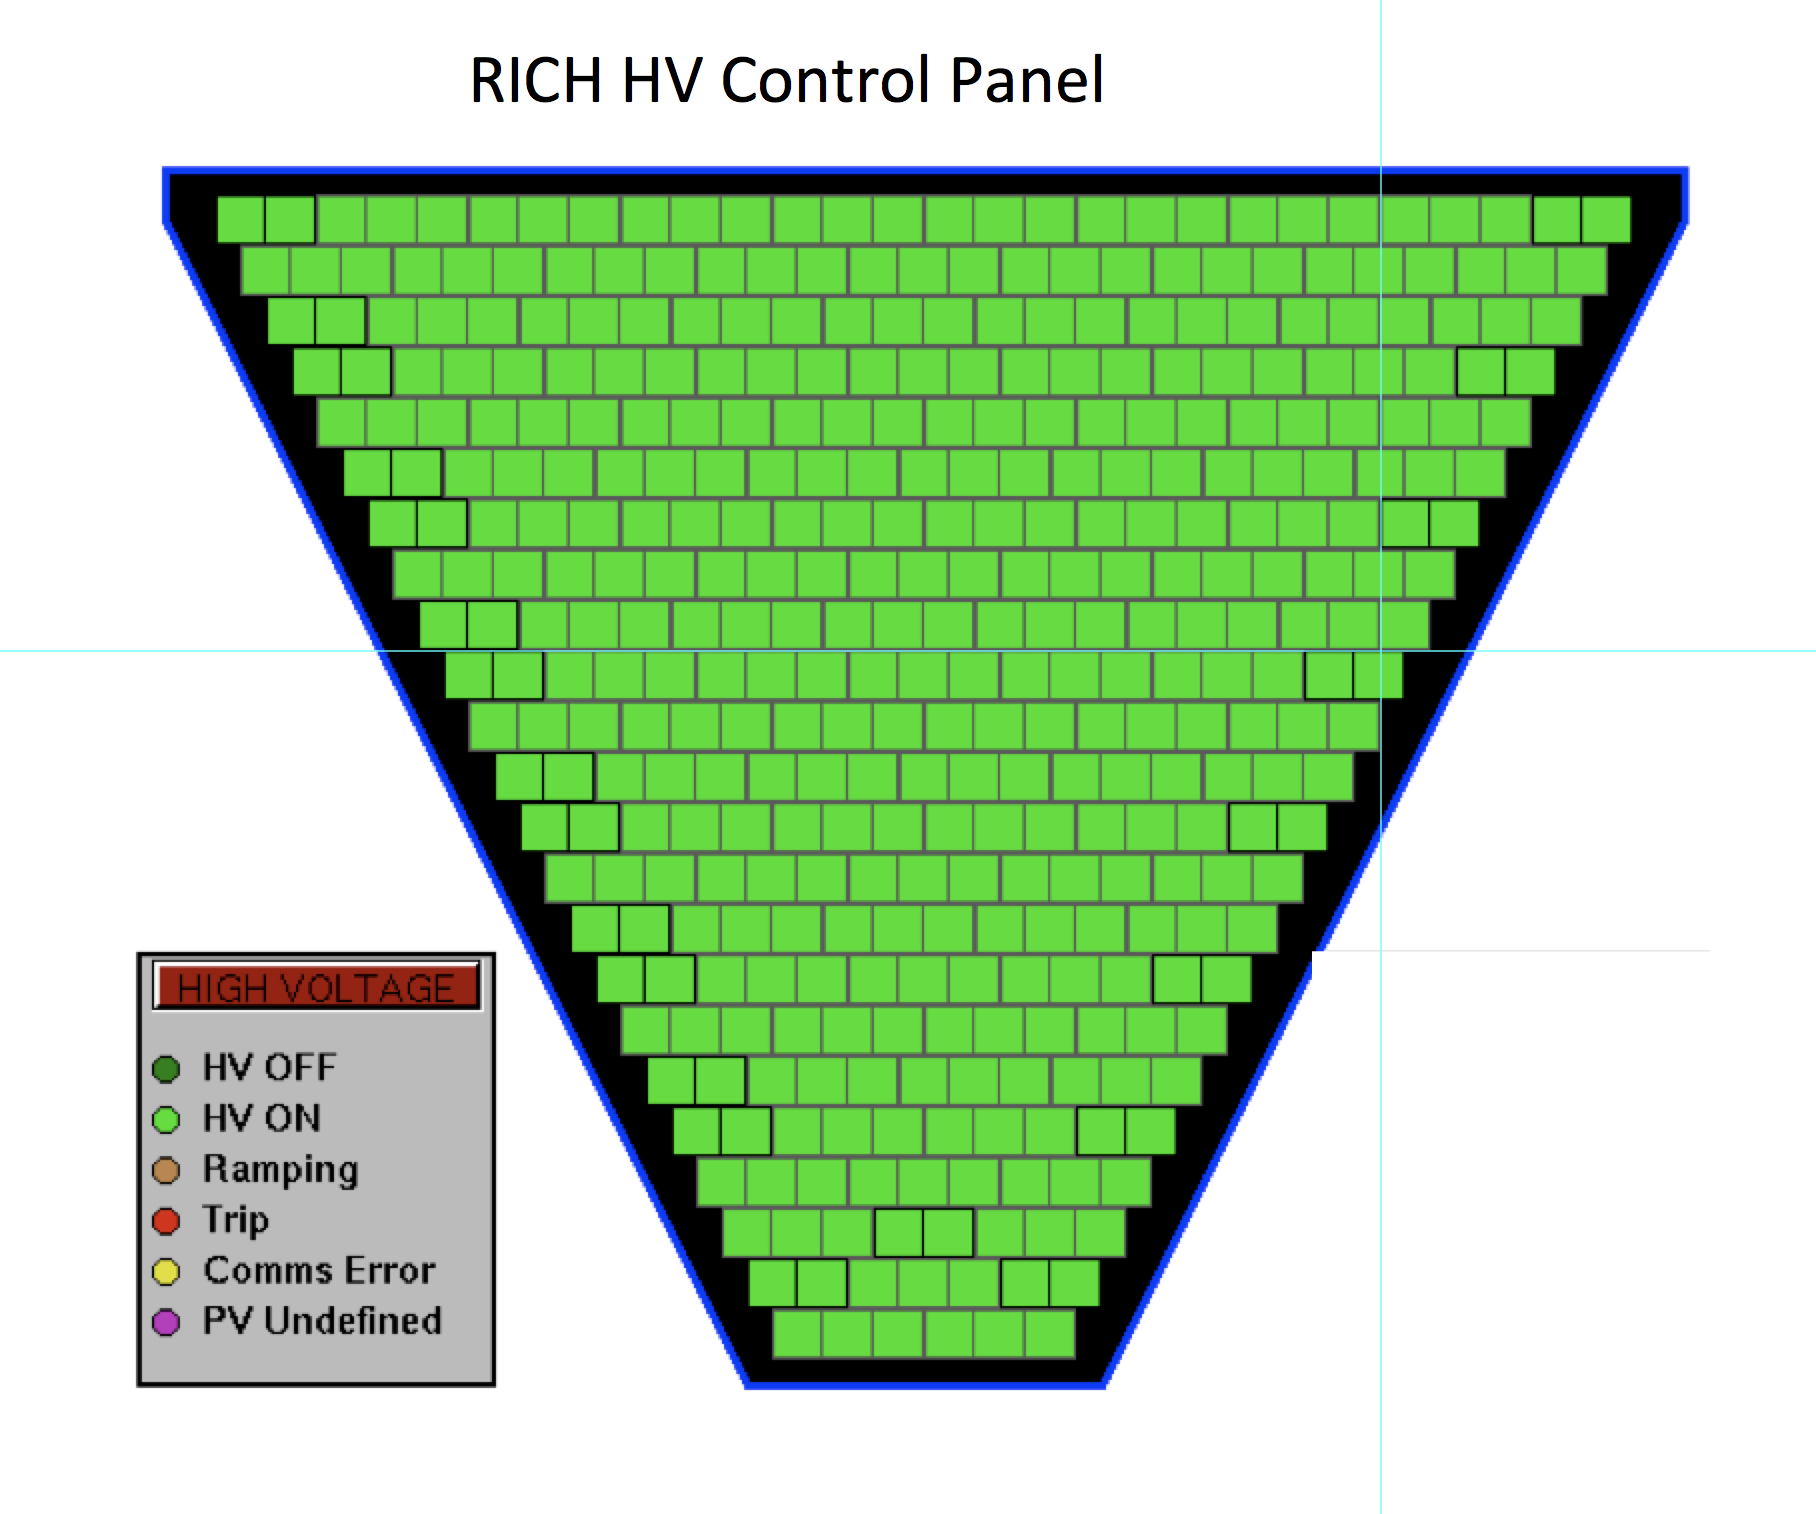
\includegraphics[width=0.95\textwidth]{pics/RICH_HV_control.png}
%\includegraphics[width=0.95\textwidth]{pics/ecalhv_2014_12_15_16:02:54.png}
\caption{ \label{HV} View of the EPICS RICH HV expert monitoring window.}
\end{figure}

%\begin{figure}[htbp]
%\center
%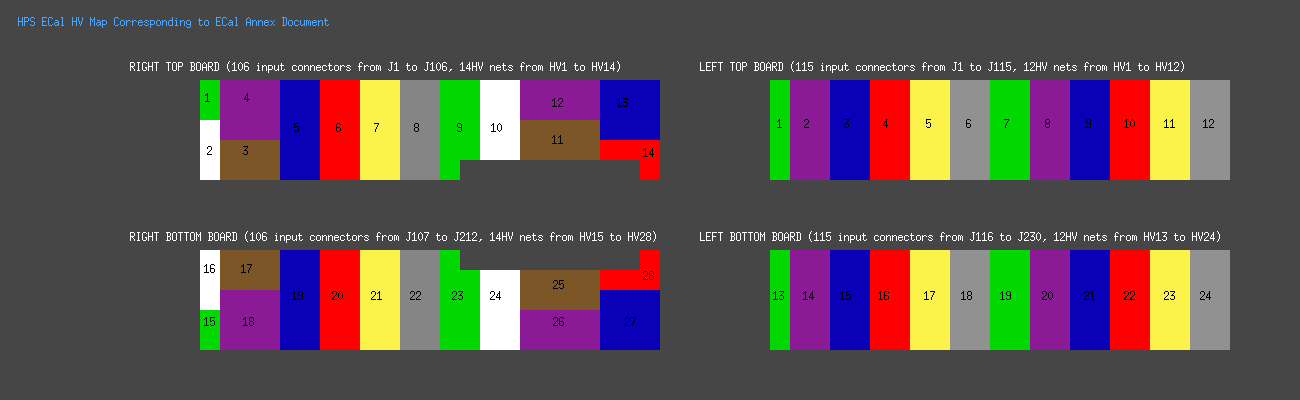
\includegraphics[width=0.95\textwidth]{pics/ecalhv_expertmap_2014_12_15.png}
%\caption{ \label{ExpertMap} Expert HV channel map for reference.}
%\end{figure}

    
      \subsubsection{HV Save/Restore}
      A system to save and restore the entire RICH's voltage settings is available via buttons in the RICH HV expert window in Figure \ref{HV}.  If the voltage setpoints are changed, a backup should be made of the new settings.  This must be run as a user in group \texttt{clas-4};  user \texttt{hpsrun} does not have sufficient priveleges to save/restore voltage settings. 
      An example of the restore window is shown in figure~\ref{fig:hvrestore}, which is accessible from the HV expert screen shown in Figure~\ref{HV}.

\begin{figure}[htbp] \centering
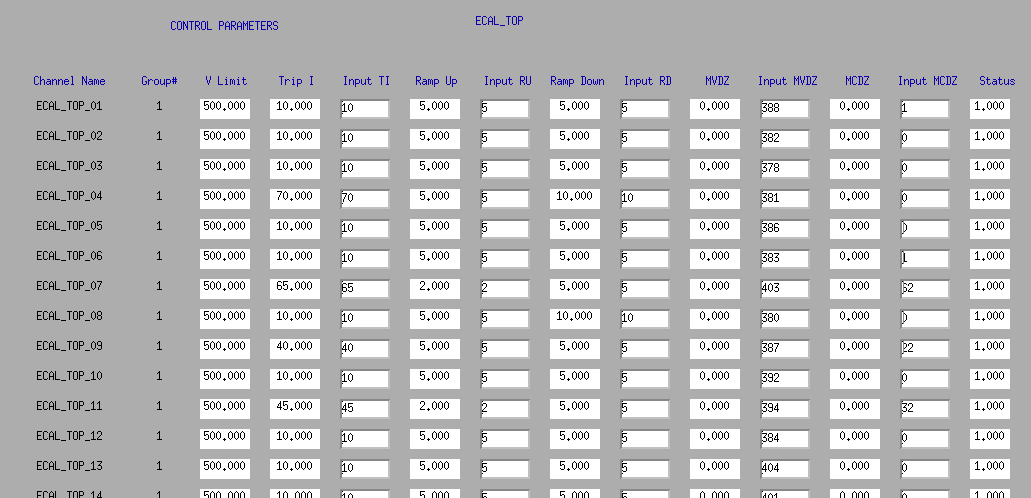
\includegraphics[width=0.85\textwidth]{pics/ecalhv_parameters_2014_12_15.png}
\caption{ \label{EHV} Cropped view of the EPICS HV expert control window. It is accessed from the parameters button in the RICH HV control screen \ref{HVControl}}
\end{figure}

\begin{figure}[htbp]\centering
    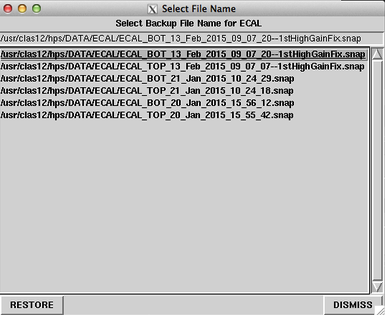
\includegraphics[width=8cm]{pics/hvrestore.png}
    \caption{The gui interface to save/restore HV settings.  \label{fig:hvrestore}}
\end{figure}

   \subsection{Long Term HV monitoring}

   An hourly snapshot of HV currents is stored by a cron job (and in the EPICs and MYA databases).  Currently the easiest way to view it is as user \texttt{clasrun} on \texttt{clonpcNN} by excuting the command:
   \begin{center}
   \texttt{\$HOME/.ecalhv/plotRICHHV.py}
   \end{center}
The product should be a plot like figure~\ref{HVhistory}.

\begin{figure}[htbp] \centering
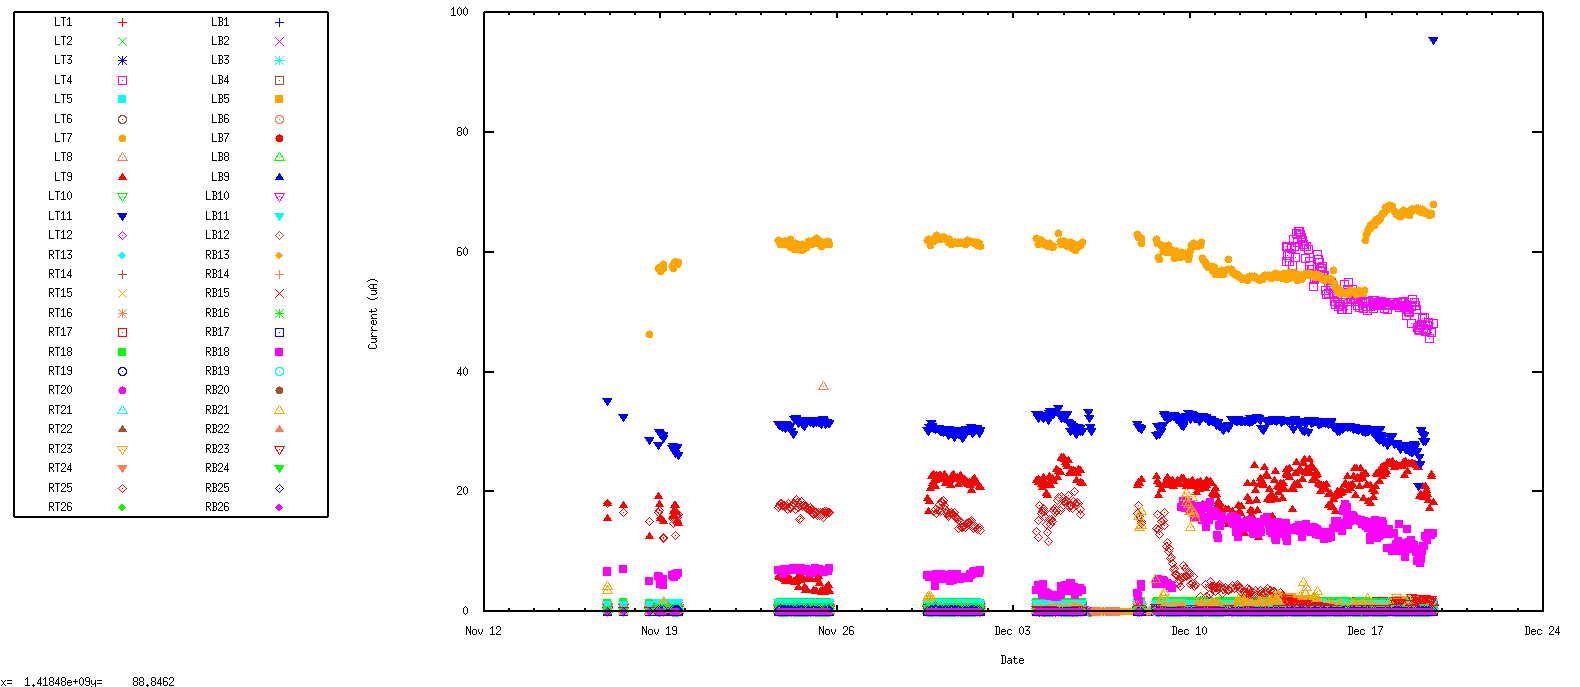
\includegraphics[width=0.95\textwidth]{pics/ECALHVCURRENTS_2014_12_20.png}
\caption{ \label{HVhistory} Expert HV current history.}
\end{figure}


%{\color{blue}
%\section{Channel Mapping GUI}
%}
%Channel mapping is available in a spreadsheet in the annex pdf on the CLAS Run Wiki. It is also available in an interactive GUI (shown in Figure \ref{fig:kylesGui}) which can be run by executing \begin{center}\texttt{kylesGui.sh}\end{center} in a terminal.

%\begin{figure}[htbp]\centering
%    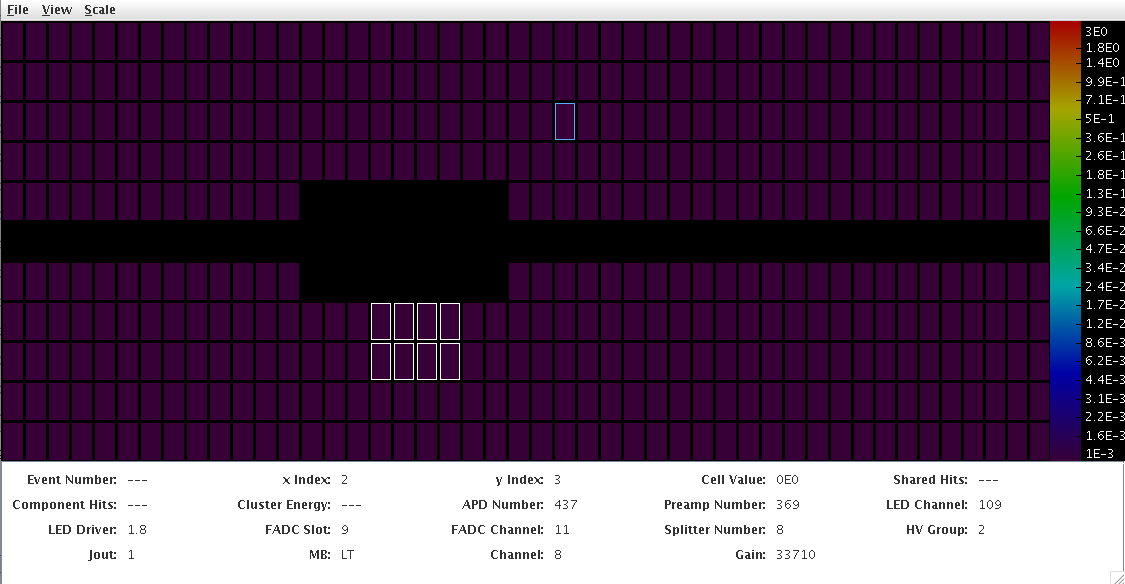
\includegraphics[width=16cm]{pics/kylesGui.png}
%    \caption{The ECal event display can be used to get channel mappings.  The blue-highlighted channel's mappings are shown in the table.  The white-highlighted channels correspond to the filtering applied via the {\bf View} menu, in this case HV group 25 on bottom.\label{fig:kylesGui}}
%\end{figure}
%%%%%%%%%%%%%%%%%%%%%%%%%%%%%%%%%%%%%%%%%%%%%%%%%%%%%%%%%%%%%%%%%%%%%%%%%%%%%
%%%%%%%%%%%%%%%%%%%%%%%%%%%%%%%%%%%%%%%%%%%%%%%%%%%%%%%%%%%%%%%%%%%%%%%%%%%%%
%%%%%%%%%%%%%%%%%%%%%%%%%%%%%%%%%%%%%%%%%%%%%%%%%%%%%%%%%%%%%%%%%%%%%%%%%%%%%
%%%%%%%%%%%%%%%%%%%%%%%%%%%%%%%%%%%%%%%%%%%%%%%%%%%%%%%%%%%%%%%%%%%%%%%%%%%%%
%%%%%%%%%%%%%%%%%%%%%%%%%%%%%%%%%%%%%%%%%%%%%%%%%%%%%%%%%%%%%%%%%%%%%%%%%%%%%
%%%%%%%%%%%%%%%%%%%%%%%%%%%%%%%%%%%%%%%%%%%%%%%%%%%%%%%%%%%%%%%%%%%%%%%%%%%%%

\iffalse

\section{Opening the Calorimeter}

This requires 2 people.  Care must be taken for all cabling during this process, including LV, HV, signal, and thermocouples.  The required tools are shown in Table ~\ref{tab:tools}.  The blue-handled chain-winches and metric crescent wrenches should be in the HPS cabinet on the pie tower.  The rest should be retrieved from the toolboxes on the Hall-B floor.  While one can get by with only half the number of wrenches of each type, it is fastest to have the full list. 

\begin{table}[htbp]\centering
    \begin{tabular}{c|l}\hline
        Count & Type \\\hline
4&   ECAL-ONLY chain winches (blue-handled)\\
4&   15/16" crescent wrenches for rod bolts\\
2&   11 mm crescent wrenches for lateral cossbar supports (over beampipe)\\
2&   6 mm hex/allen wrenches for longitudinal crossbar supports (on far left/right)\\
2&   3/16" hex/allen wrenches for support plates\\
2&   medium-sized flathead screwdrivers\\\hline
    \end{tabular}
    \caption{Items used to open the calorimeter. \label{tab:tools}}
\end{table}

{\bf\em PLEASE return ALL tools back to where you found them.}

   \section{Disconnection of a Channel and Preamplifier Replacement}
     
      In last resort, to recover a HV group that is tripping one can disconnect the faulty channel causing trouble. To do so, you need to find exactly which channel is involved! It might be obvious from data, if the channel was already very noisy, else you will have to test the channels of the group one by one. This is a lengthy operation and should only be attempted with the authorization of the run coordinator and in coordination with the ECal Group. It necessitates that the Hall-B crew moves the ECal out of the beam line and to open it.

   \section{LED system for experts}

This section has to be replaced with instructions to use the CLAS\_css GUI.

\begin{figure}[htbp]
\center
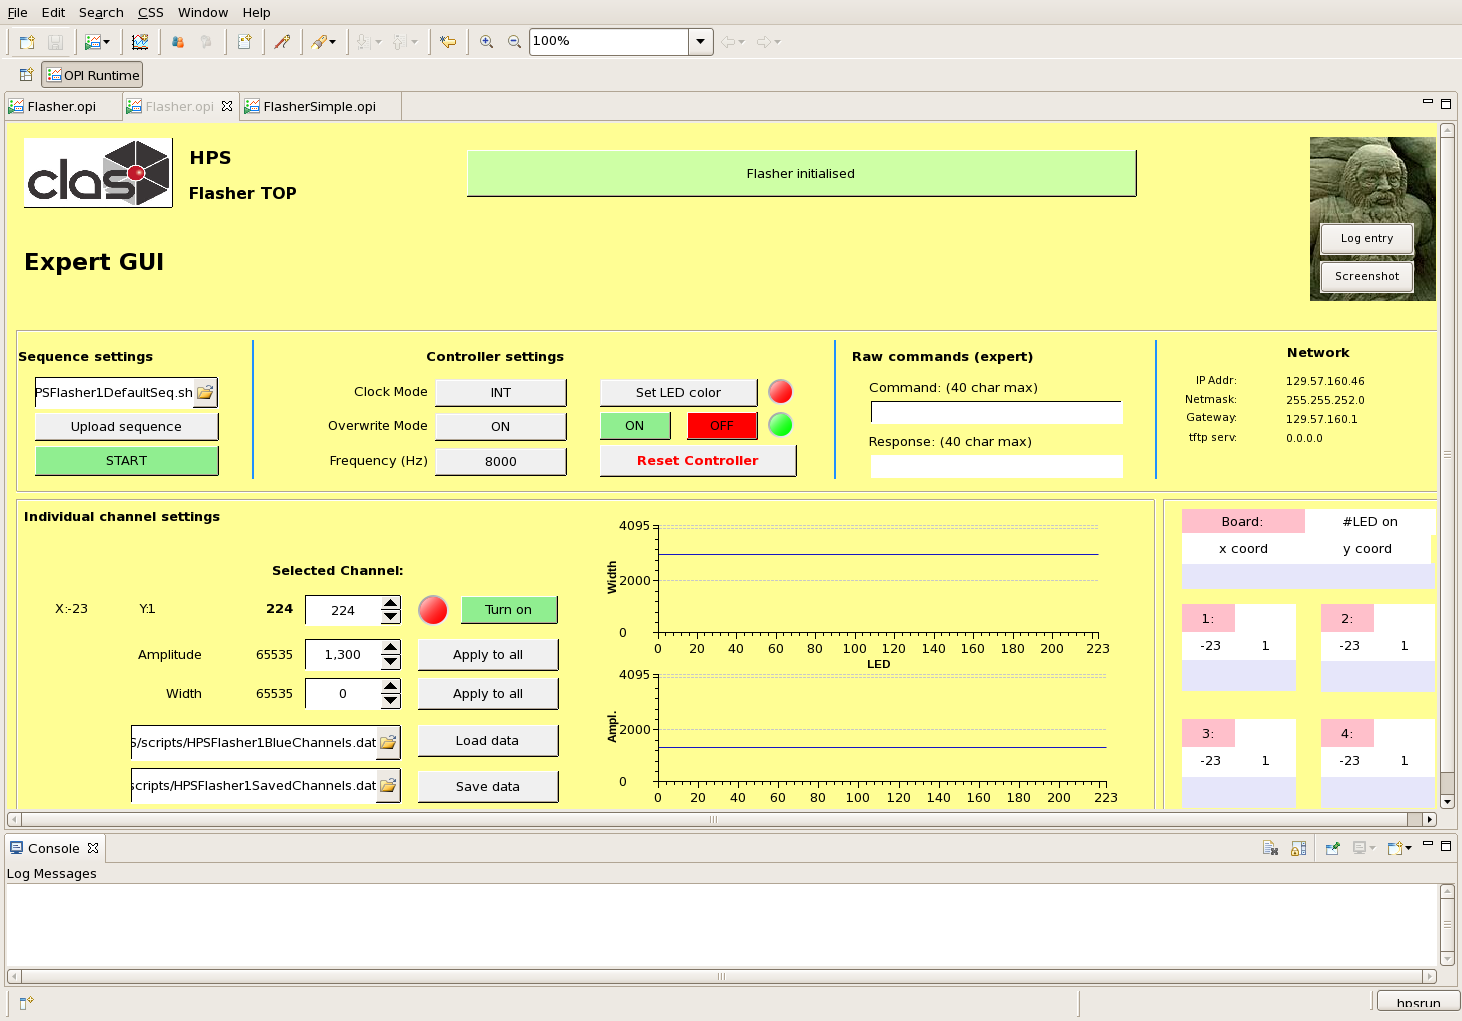
\includegraphics[width=0.85\textwidth]{pics/LEDExpert_2014_12_20.png}
\caption{\label{LEDexpert} View of the LED expert controls.}
\end{figure}
%%%%%%%%%%%%%%%%%%%%%%%%%%%%%%%%%%%%%%%%%%%%%%%%%%%%%%%%%%%%%%%%%%%%%%%%%%%%%
%%%%%%%%%%%%%%%%%%%%%%%%%%%%%%%%%%%%%%%%%%%%%%%%%%%%%%%%%%%%%%%%%%%%%%%%%%%%%
%%%%%%%%%%%%%%%%%%%%%%%%%%%%%%%%%%%%%%%%%%%%%%%%%%%%%%%%%%%%%%%%%%%%%%%%%%%%%
%%%%%%%%%%%%%%%%%%%%%%%%%%%%%%%%%%%%%%%%%%%%%%%%%%%%%%%%%%%%%%%%%%%%%%%%%%%%%
%%%%%%%%%%%%%%%%%%%%%%%%%%%%%%%%%%%%%%%%%%%%%%%%%%%%%%%%%%%%%%%%%%%%%%%%%%%%%
%%%%%%%%%%%%%%%%%%%%%%%%%%%%%%%%%%%%%%%%%%%%%%%%%%%%%%%%%%%%%%%%%%%%%%%%%%%%%
\fi
\end{document}
